\Chapter{Evaluation and experimentation}

\section{Technical aspects of the implementation}

The SOAR cognitive architecture yields itself well to implementation using Entity-Component-System (ECS) approach.
The ECS pattern is a data-driven approach to game implementation where all logic is implemented as either components or systems \cite{raffaillac2019polyphony}.
An entity is a collection of components which in turn are containers of data that hold some state but no logic of their own.
The systems are functions that operate on entities based on some defined queries (such as all entities containing a component representing position and velocity) and then modify the state of the components.
This approach is performant as it allows for many otherwise impossible optimization techniques to be utilized (such as SIMD instructions and aggresive inlining)\cite{harkonen2019advantages}.
In the case of the cognitive architecture in question, the components would be working memory elements as well as inference and behaviour rules.
A sensory system could be designed for feeding the working memory with the state of the world based on other components such as position, state, health or other types of data.
Another set of systems would run all inference rules and behaviour rules and finally a system would evaluate operators proposed by the previous system and execute their actions.

The actual implementation of all simulations in this thesis is based on the MonoGame framework as described in the book "Introducing 2D Game Development in C\#"\cite{pavleas2013introducing}.
The ECS implementation used "a high-performance C\# based Archetype and Chunks Entity Component System (ECS) for game development and data-oriented programming" called Arch\cite{matthaeus2023arch}.
The reason for choosing this project over others is due to the results of performance analysis done by Paillat Laszlo in their ECS benchmark\cite{laszlo2023arch}.

\section{Implementation of infection model}

Social media and information propagation are similar in nature to epidemiological phenomena.
It is common to refer to a fast spreading news as being viral, referring to its ability to spread from host to host rapidly.
In epidemiology the simplest approach to model how a disease spreads is to use a compartmental model that divides the population into compartments or categories and then assigns each compartment a mathematical description of its population size over time.
Modelling the spread of infectious diseases has long been the goal of many scientists\cite{liu2016}.
The simplest and most popular model is based on the partitioning of a population in three compartments of susceptible, infected and recovered\cite{weiss2013sir}.
This model is called SIR and consists of three differential equations describing each compartment.
Figure \ref{fig:sir.drawio.png} illustrates possible state transitions within the SIR model.

\begin{figure}[H]
    \centering
    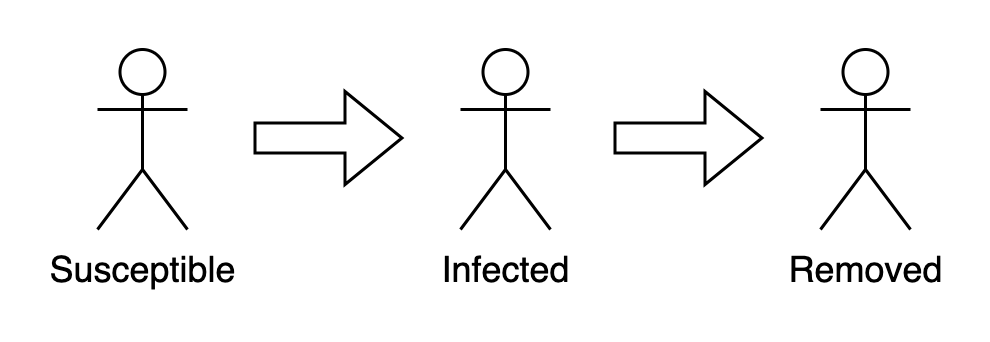
\includegraphics[width=0.6\textwidth]{images/chapter2/sir.drawio.png}
    \caption{Agent state transition in SIR model}\label{fig:sir.drawio.png}
\end{figure}

\begin{equation} \label{eq:sir1}
    \frac{{dS}}{{dt}} = -\frac{{\beta \cdot S \cdot I}}{{N}}
\end{equation}

\begin{equation} \label{eq:sir2}
    \frac{{dI}}{{dt}} = \frac{{\beta \cdot S \cdot I}}{{N}} - \gamma \cdot I
\end{equation}

\begin{equation} \label{eq:sir3}
    \frac{{dR}}{{dt}} = \gamma \cdot I
\end{equation}

Equations \ref{eq:sir1}, \ref{eq:sir2} and \ref{eq:sir3} describe how each compartment of the population changes over time.
The parameters of the model are:

\begin{itemize}
    \item $S$: Number of susceptible individuals in the population
    \item $I$: Number of infected individuals
    \item $R$: Number of recovered individuals
    \item $N$: Total population size ($N = S + I + R$)
    \item $\beta$: Infection rate, determining the probability of a susceptible individual becoming infected when coming into contact with an infected individual
    \item $\gamma$: Recovery rate, indicating the average rate at which infected individuals recover and become immune
\end{itemize}

Variations of this model exist that aim to improve its representativeness in the real world usually by adding another partition group such as hibernator in SIHR\cite{zhao2012sihr}.
While the origins of these models stems from simulation of infectious diseases spreading across a population, many authors realized that social media and rumors can be modelled exactly the same way.
The SIHR model for instance is an example of a "rumor spreading model in social networks"\cite{zhao2012sihr}.
Another variant of the simple SIR model is SCIR, in which the letter 'C' stands for contacted and 'R' stands for refractory.
This model is used to analyze the impact of the "retweeting mechanism for online social media"\cite{xiong2012scir}.
Some authors use the concept of cellular automata to implement simulations of the spread of rumors or diseases\cite{silva2020}.
Because the name of the last group "recovered" is more strongly associated with diseases and epidemiological modelling, in this thesis a more general naming was adapted and the last group is called "removed" to indicate that the members of the population within that compartment do not take part in the simulation anymore.

Because the scope of this thesis is limited to application of such models in games, the aim of the proposed model is not to be as accurate in representation of real world disease spread but to be able to represent the idea behind modelling the spread of rumors or diseases in video games.
The most important aspect of the evaluation is the ability to express the standard SIR model using the cognitive architecture proposed in the preceding chapter.
For this reason a population is a multi-agent system where each agent can be susceptible or infected.
The agents have two defined behaviour rules.
The first one can be summarized as "if not in contact with previously uncontacted agent and possessing message, go towards closest uncontacted agent".
Whereas second one is "if in contact with previously uncontacted agent and possessing message, make contact".
The action of contact is modelled using the $Tell$ operator with an arbitrary message.
The message plays no special role in the simulation and instead represents either a rumor or a disease being spread.
The condition that checks for the possession of the message is the one that differentiates infected agents from susceptible ones.
It is worth to note that in order for the simulation to produce any results, at least one agent must be initialized with the possession of the message (infection).
In general the logic expressed by the combination of previously defined behaviour and inference rules can be illustrated using a flowchart shown in figure \ref{fig:sir_logic.drawio.png}.

\subsection{Experiment 1}

\begin{figure}[h]
    \centering
    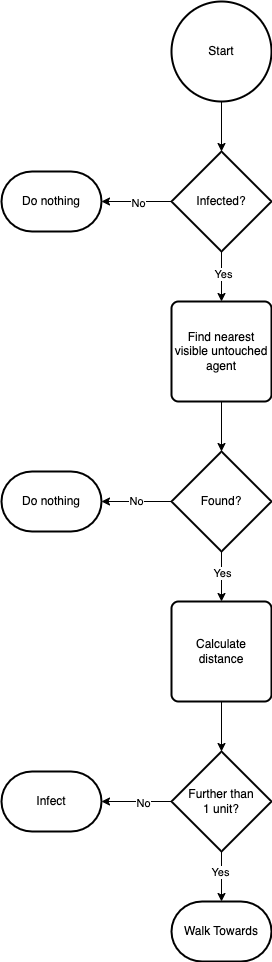
\includegraphics[width=0.6\textwidth]{images/chapter2/sir_logic.drawio.png}
    \caption{Flowchart representing logic expressed by agent behaviour rules, terminal blocks represent operators being proposed by the agent}\label{fig:sir_logic.drawio.png}
\end{figure}

The simulation starts with a single agent being infected and the rest of the agents randomly distributed in a rectangular area.
The initial state is visible on figure \ref{fig:images/chapter2/sir0/sir_1.png}.
The first experiment assumes each agent can see other agents that are up to 8 tiles away from it and that no agent can ever become removed.
Immedietly in the second step of the simulation, the infected agent met up with an adjacent agent and infected them.
Soon after two clusters of agents formed, each with agents trying to touch each other first before moving on.
The two clusters are visible on figure \ref{fig:images/chapter2/sir0/sir_28.png}.
After 71 simulation steps nearly all agents have been infected and strong clustering behaviour is clearly visible (figure \ref{fig:images/chapter2/sir0/sir_71.png}).
Figure \ref{fig:images/chapter2/sir0/sir_85.png} shows the final state of the simulation after 85 steps where all agents have become infected and there are no remaining survivors.

\begin{figure}[H]
    \centering
    \subfigure[Step 1]{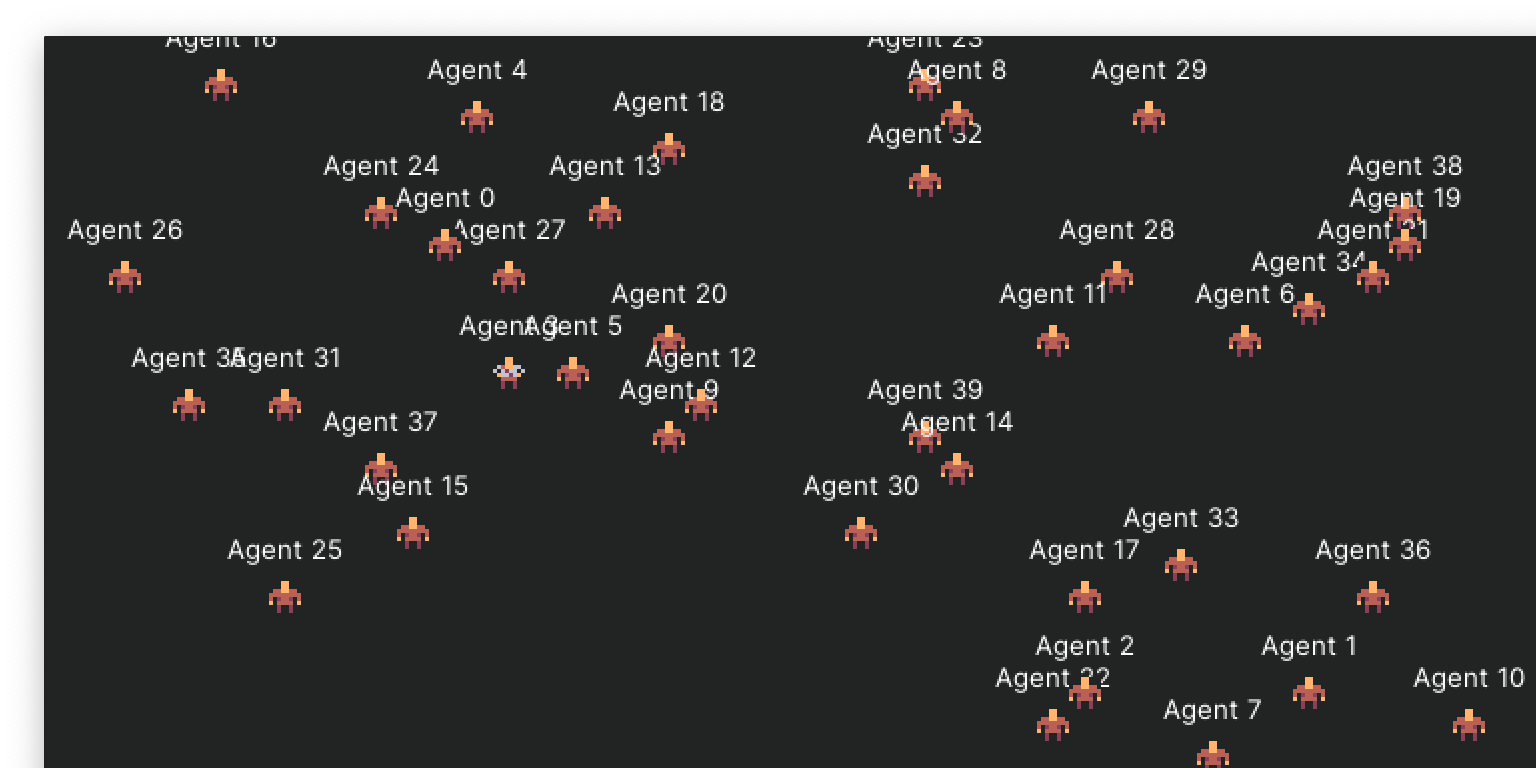
\includegraphics[width=0.48\textwidth]{images/chapter2/sir0/sir_1.png}\label{fig:images/chapter2/sir0/sir_1.png}}
    \hspace*{\fill}
    \subfigure[Step 28]{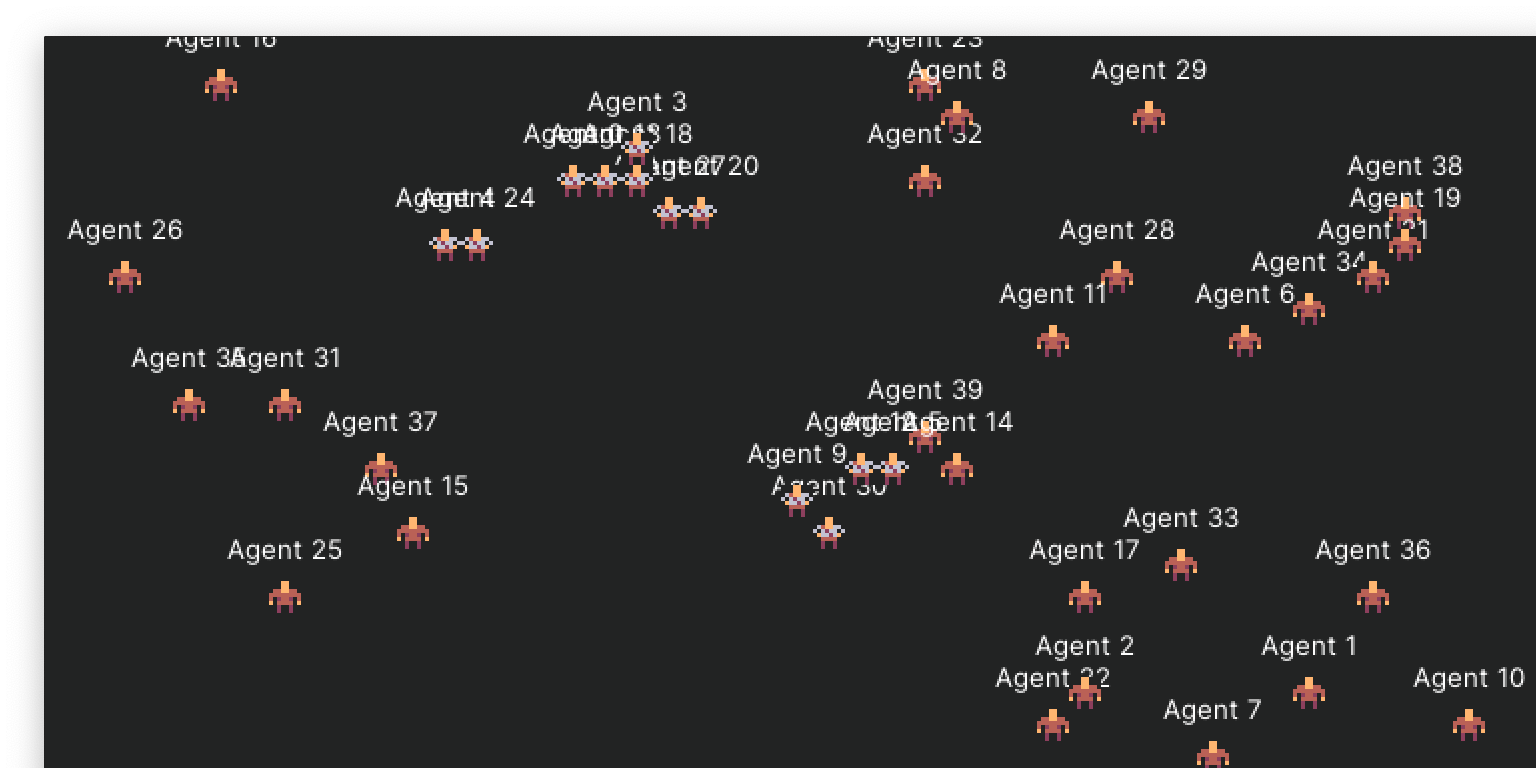
\includegraphics[width=0.48\textwidth]{images/chapter2/sir0/sir_28.png}\label{fig:images/chapter2/sir0/sir_28.png}}

    \subfigure[Step 71]{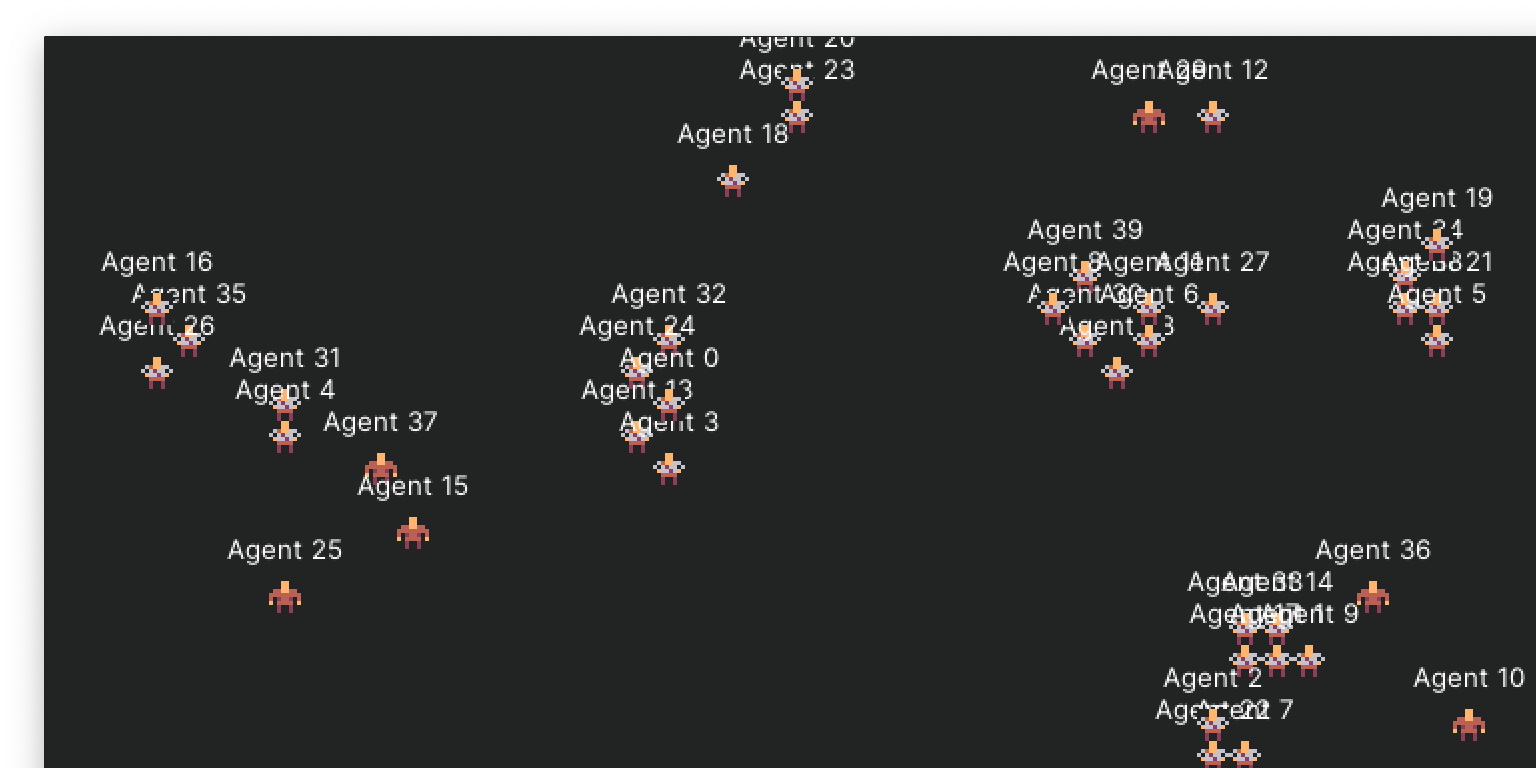
\includegraphics[width=0.48\textwidth]{images/chapter2/sir0/sir_71.png}\label{fig:images/chapter2/sir0/sir_71.png}}
    \hspace*{\fill}
    \subfigure[Step 85]{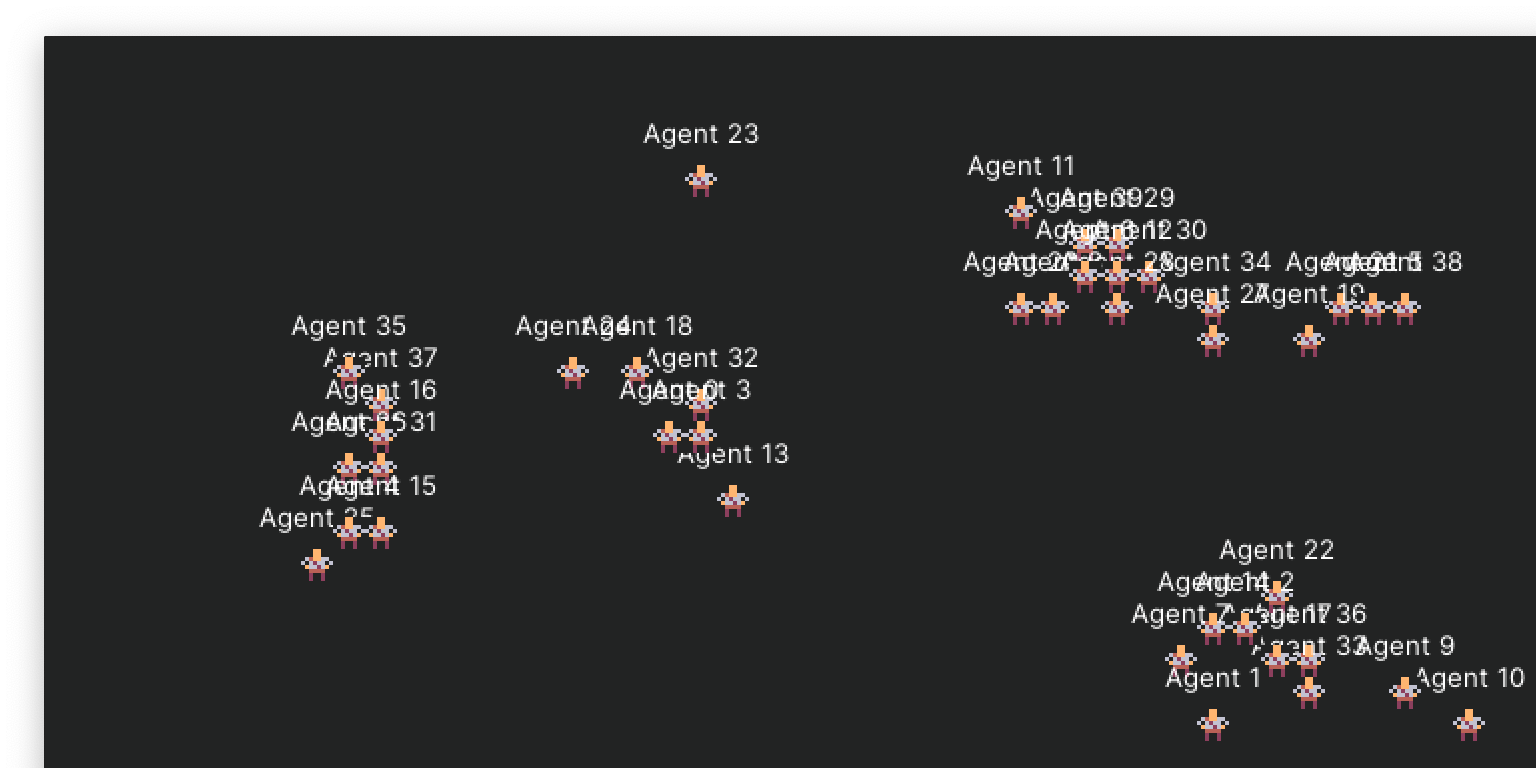
\includegraphics[width=0.48\textwidth]{images/chapter2/sir0/sir_85.png}\label{fig:images/chapter2/sir0/sir_85.png}}

    \caption{Experiment 1} \label{fig:experiment0}
\end{figure}

Due to the behaviour rule specifying that each agent should try to meet with each previously unmet agent that was seen at least once, the agents will form clusters and thus potentially separate themselves further away from other healthly individuals.
While it might seem like a strange behaviour in an epidemic model, it might make seen to consider it in terms of information propagation as humans have natural tendencies to form groups of interest.
So far the simulation assumed that agents that were not infected would remain still and do nothing.
This combined with the limited sight of the agents means that the simulation may stabilize in such a way that a survivor or group of survivors would remain undisturbed because of random distribution of agents.
An example of this situation is visible in figure \ref{fig:images/chapter2/sir0/sir_255.png}.
A slight modification of the behaviour rules will make them instead choose a random direction to go which should decrease possibility of the model stabilizing in a state where survivors remain in the simulation because no infected agent came close enough to them.

\begin{figure}[H]
    \centering
    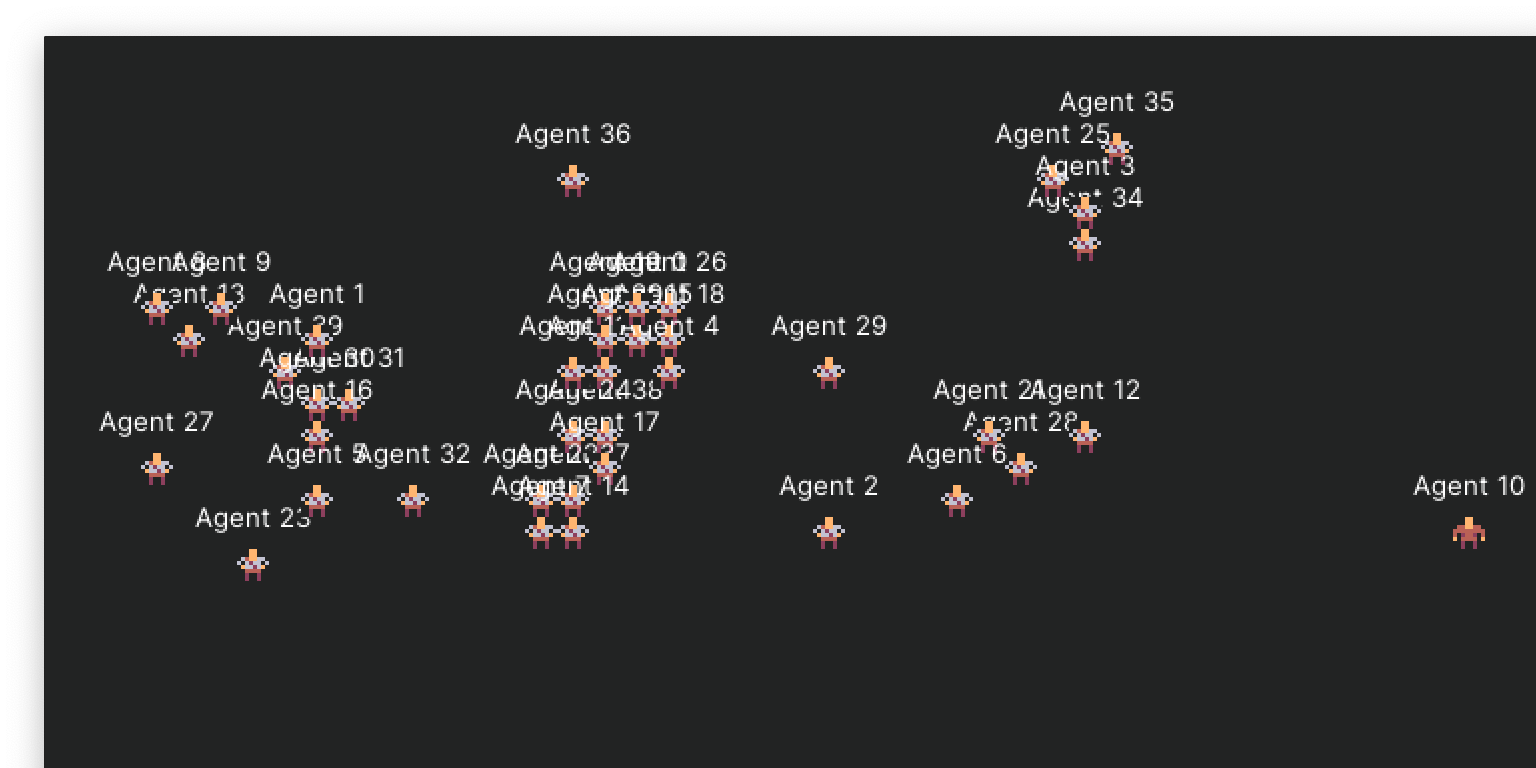
\includegraphics[width=1.0\textwidth]{images/chapter2/sir0/sir_255.png}
    \caption{Experiment 1 - lone survivor}\label{fig:images/chapter2/sir0/sir_255.png}
\end{figure}

\subsection{Experiment 2}

After modification of the behaviour rules to make susceptible individuals move around randomly as well as addition of a new rule that prevents the infected agent from targeting other infected agents the clustering behaviour is gone.
Figure \ref{fig:images/chapter2/sir1/sir_123.png} shows the final state of the experiment with the new ruleset.
The distribution of the agents is more homogeneous than before, even though slight clustering still occurs.
The population size plotted against time on figure \ref{fig:images/chapter2/sir1/sir.png} matches with the SIR model plotted on figure \ref{fig:images/chapter2/sir_ref/sir_1.png} with parameters $\beta = 0.07, \gamma = 0.0, N = 40$.

% Experiment 2

\begin{figure}[H]
    \centering
    \subfigure[Experiment]{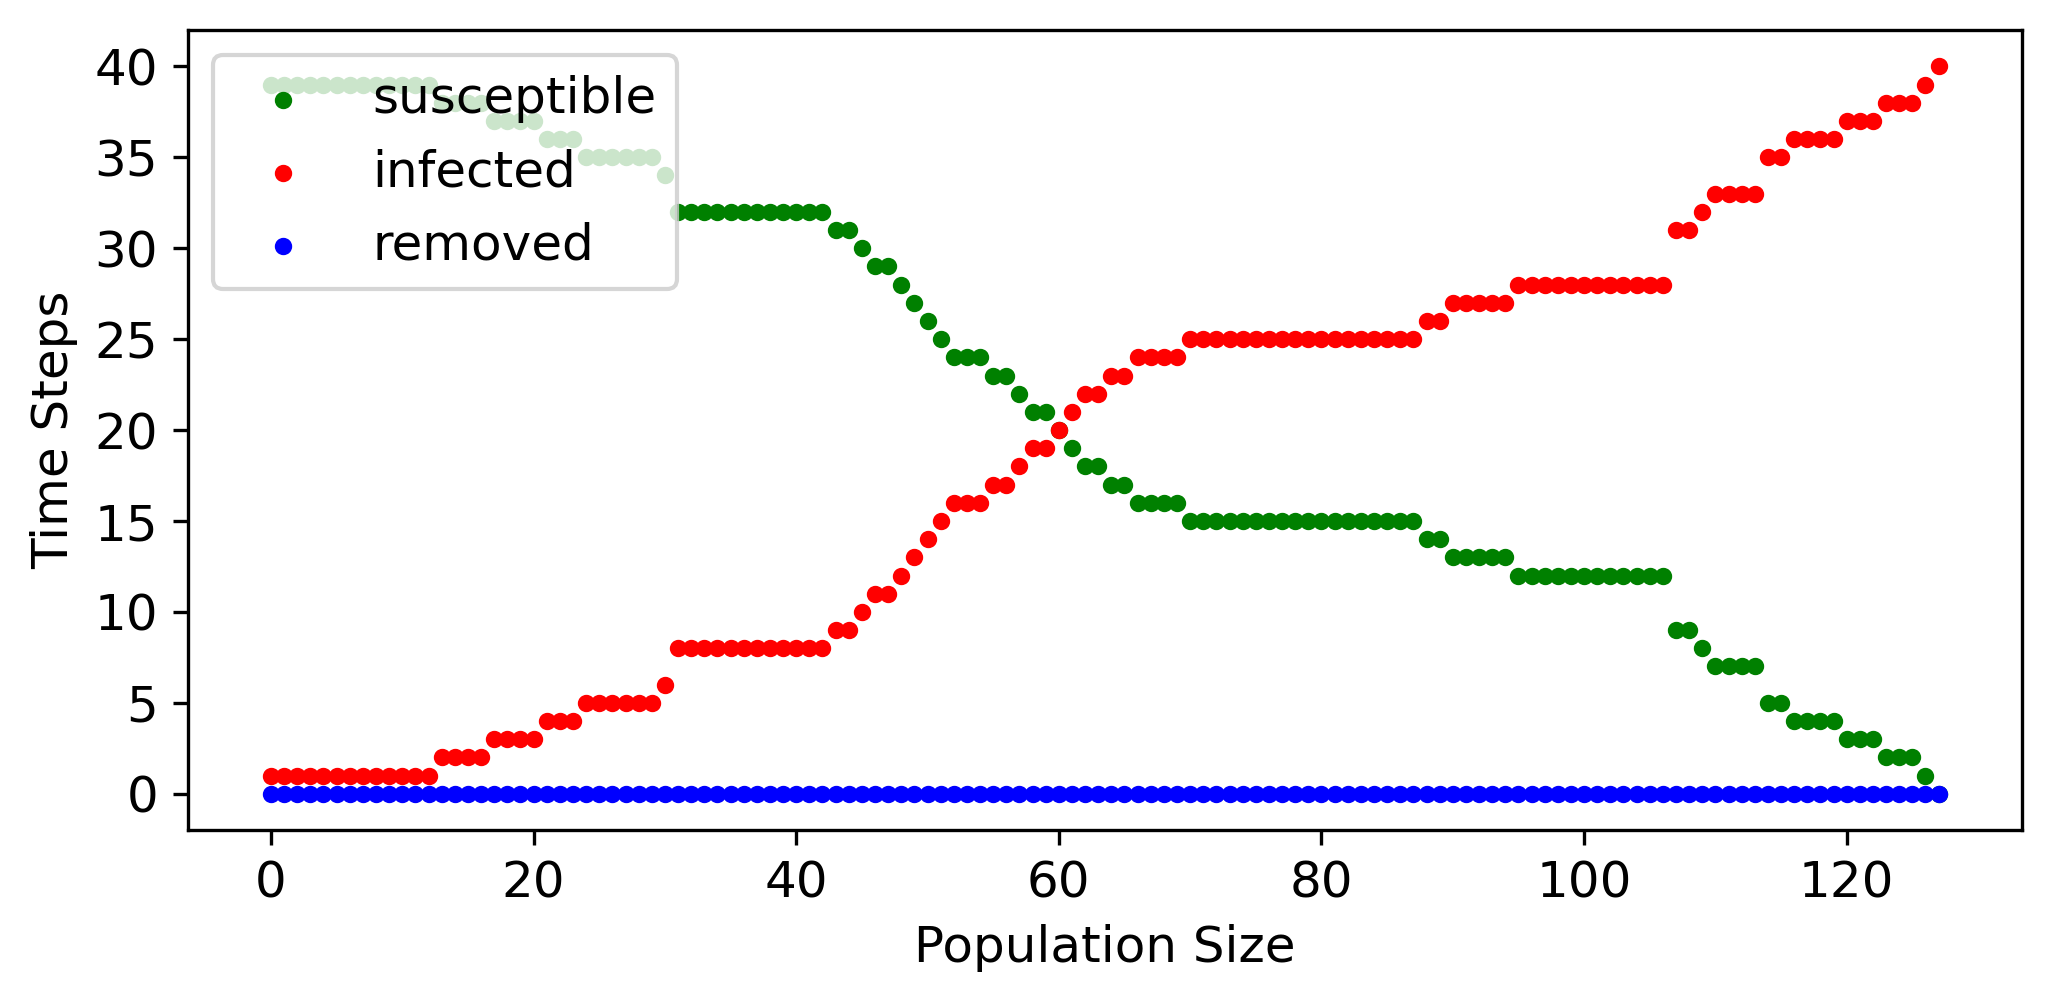
\includegraphics[width=0.48\textwidth]{images/chapter2/sir1/sir.png}\label{fig:images/chapter2/sir1/sir.png}}
    \hspace*{\fill}
    \subfigure[$\beta = 0.07, \gamma = 0.0, N = 40$]{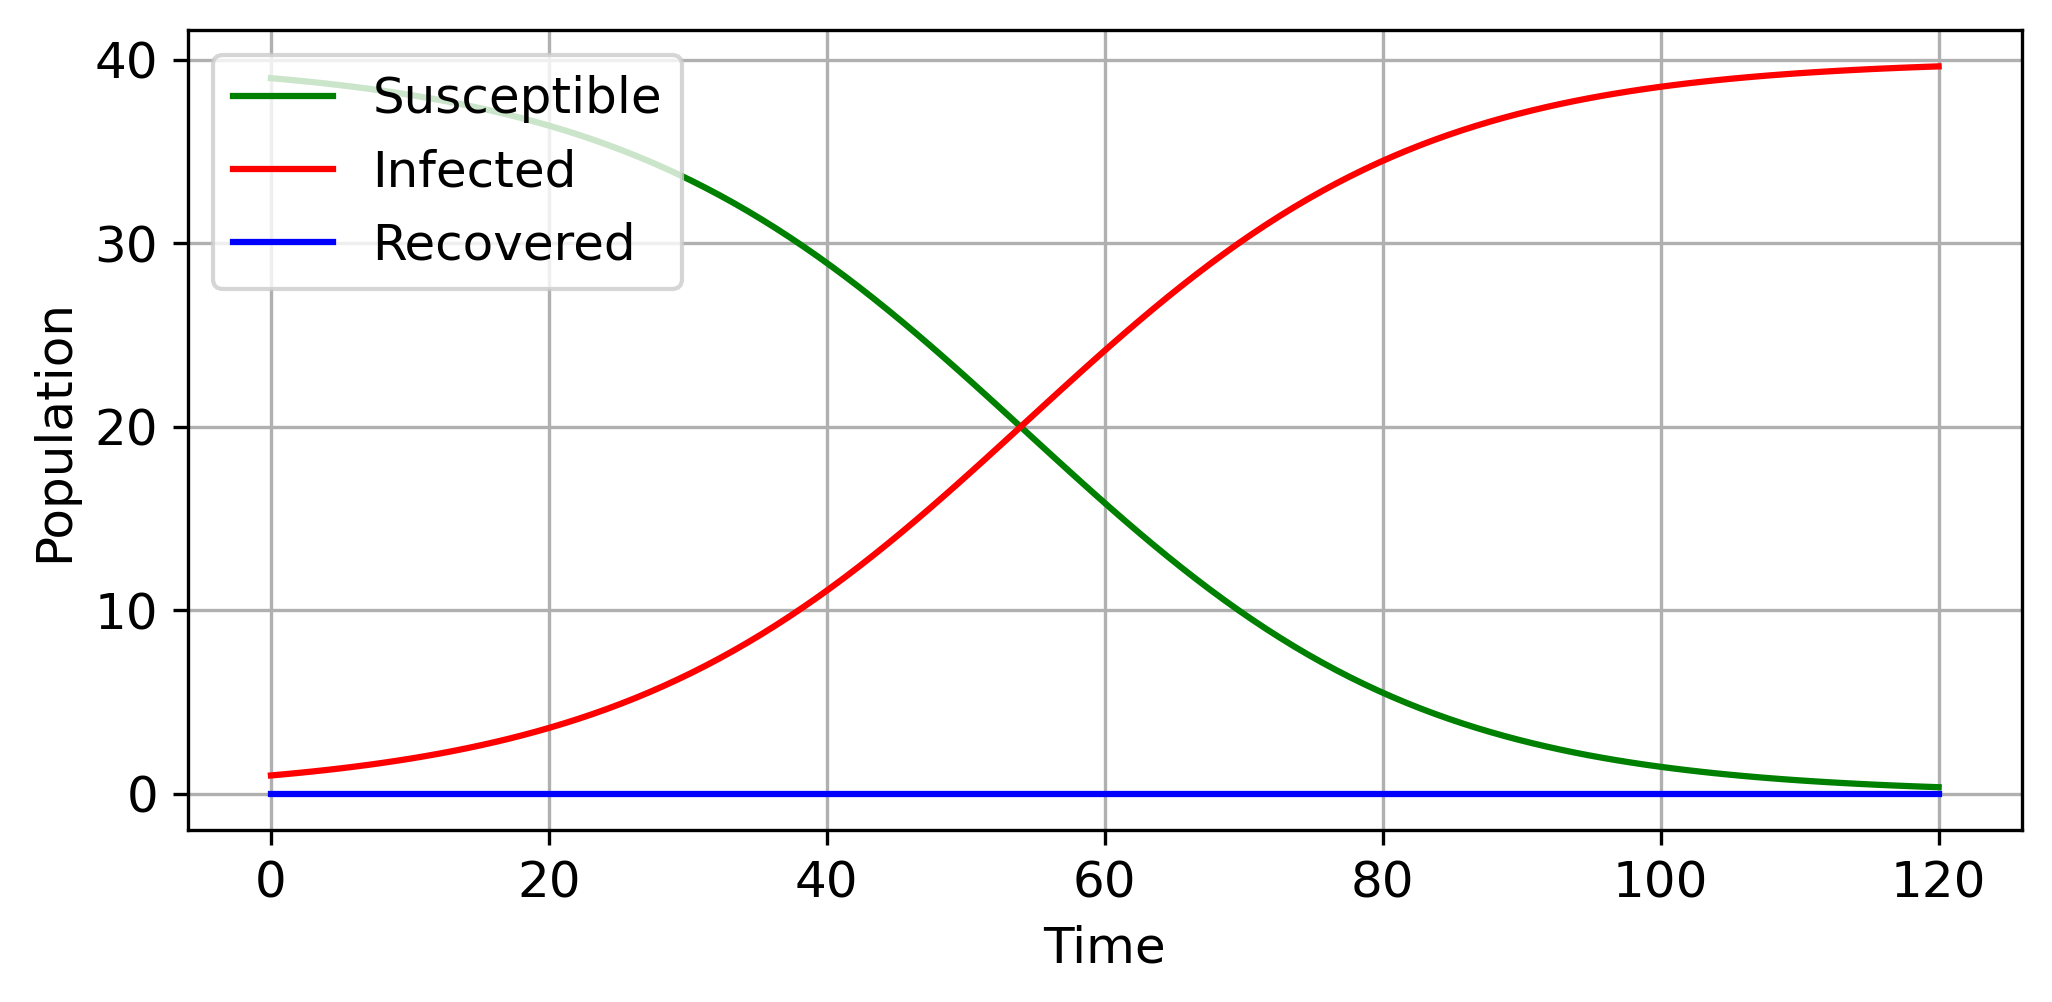
\includegraphics[width=0.48\textwidth]{images/chapter2/sir_ref/sir_1.png}\label{fig:images/chapter2/sir_ref/sir_1.png}}
    \caption{Experiment 2 - SIR vs Experiment} \label{fig:experiment1-diagrams}
\end{figure}

The initial state of the experiment shown on figure \ref{fig:images/chapter2/sir1/sir_1.png} is the same as with every other experiment.
The agents are randomly distributed and form three visually identifiable segments.
After the simulation starts infected agents quickly form a cluster in the bottom right corner as visible on figure \ref{fig:images/chapter2/sir1/sir_33.png}.
Soon after the cluster disperses and the agents move on to infect the rest of the population.
Finally, after 128 simulation steps, the whole population is infected and there are no more remaining survivors (figure \ref{fig:images/chapter2/sir1/sir_123.png}).

\begin{figure}[H]
    \centering
    \subfigure[Step 1]{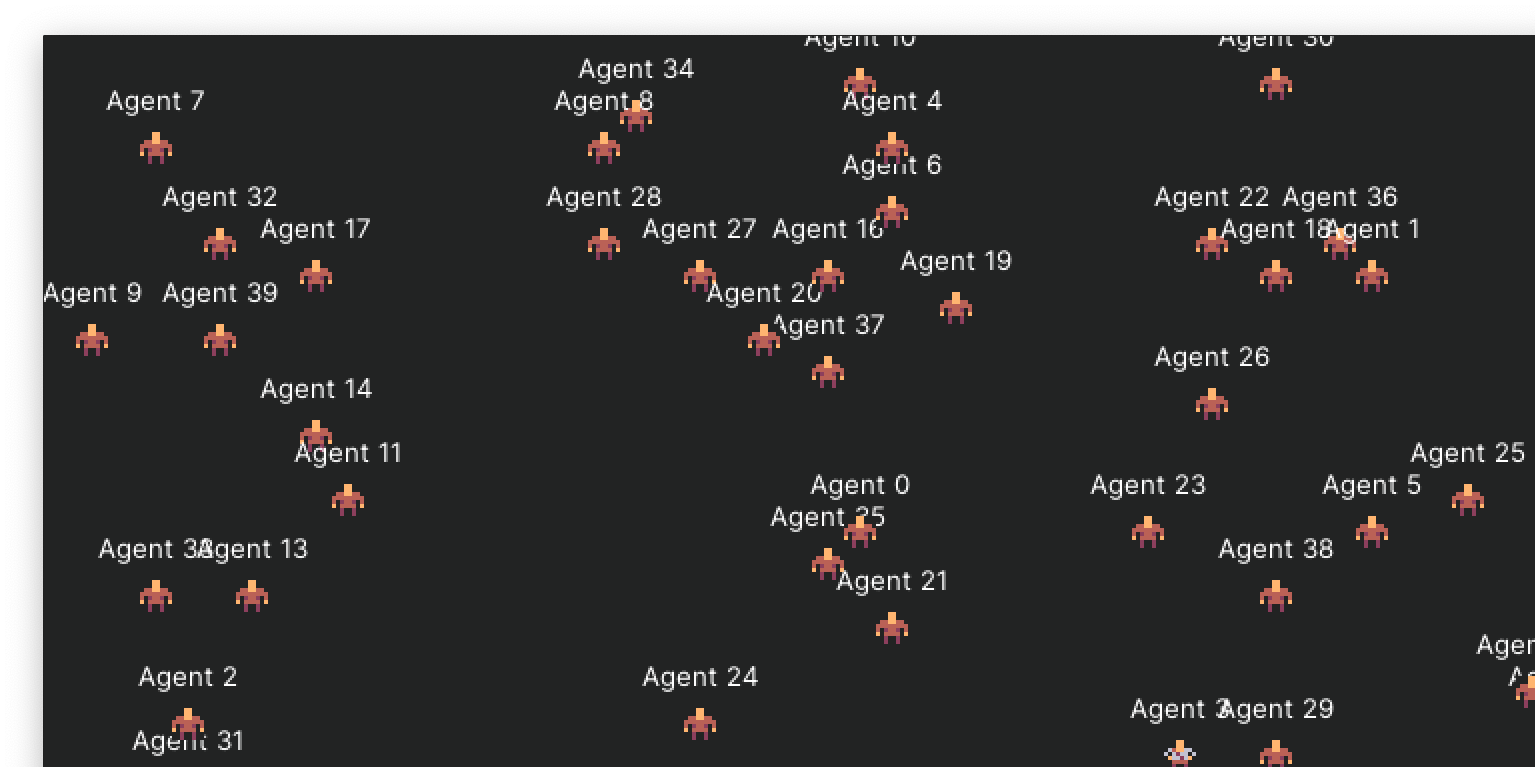
\includegraphics[width=0.3\textwidth]{images/chapter2/sir1/sir_1.png}\label{fig:images/chapter2/sir1/sir_1.png}}
    \hspace*{\fill}
    \subfigure[Step 33]{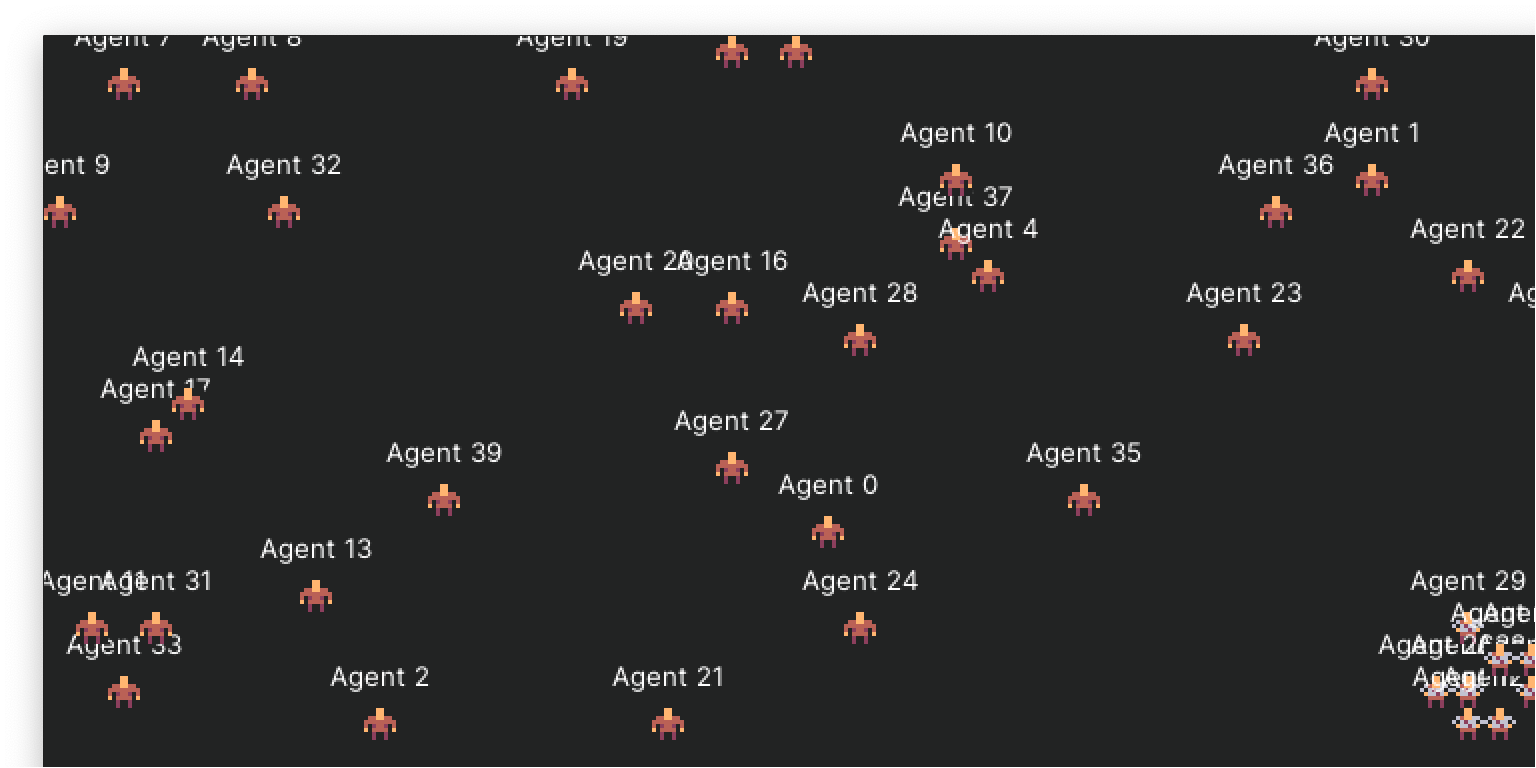
\includegraphics[width=0.3\textwidth]{images/chapter2/sir1/sir_33.png}\label{fig:images/chapter2/sir1/sir_33.png}}
    \hspace*{\fill}
    \subfigure[Step 128]{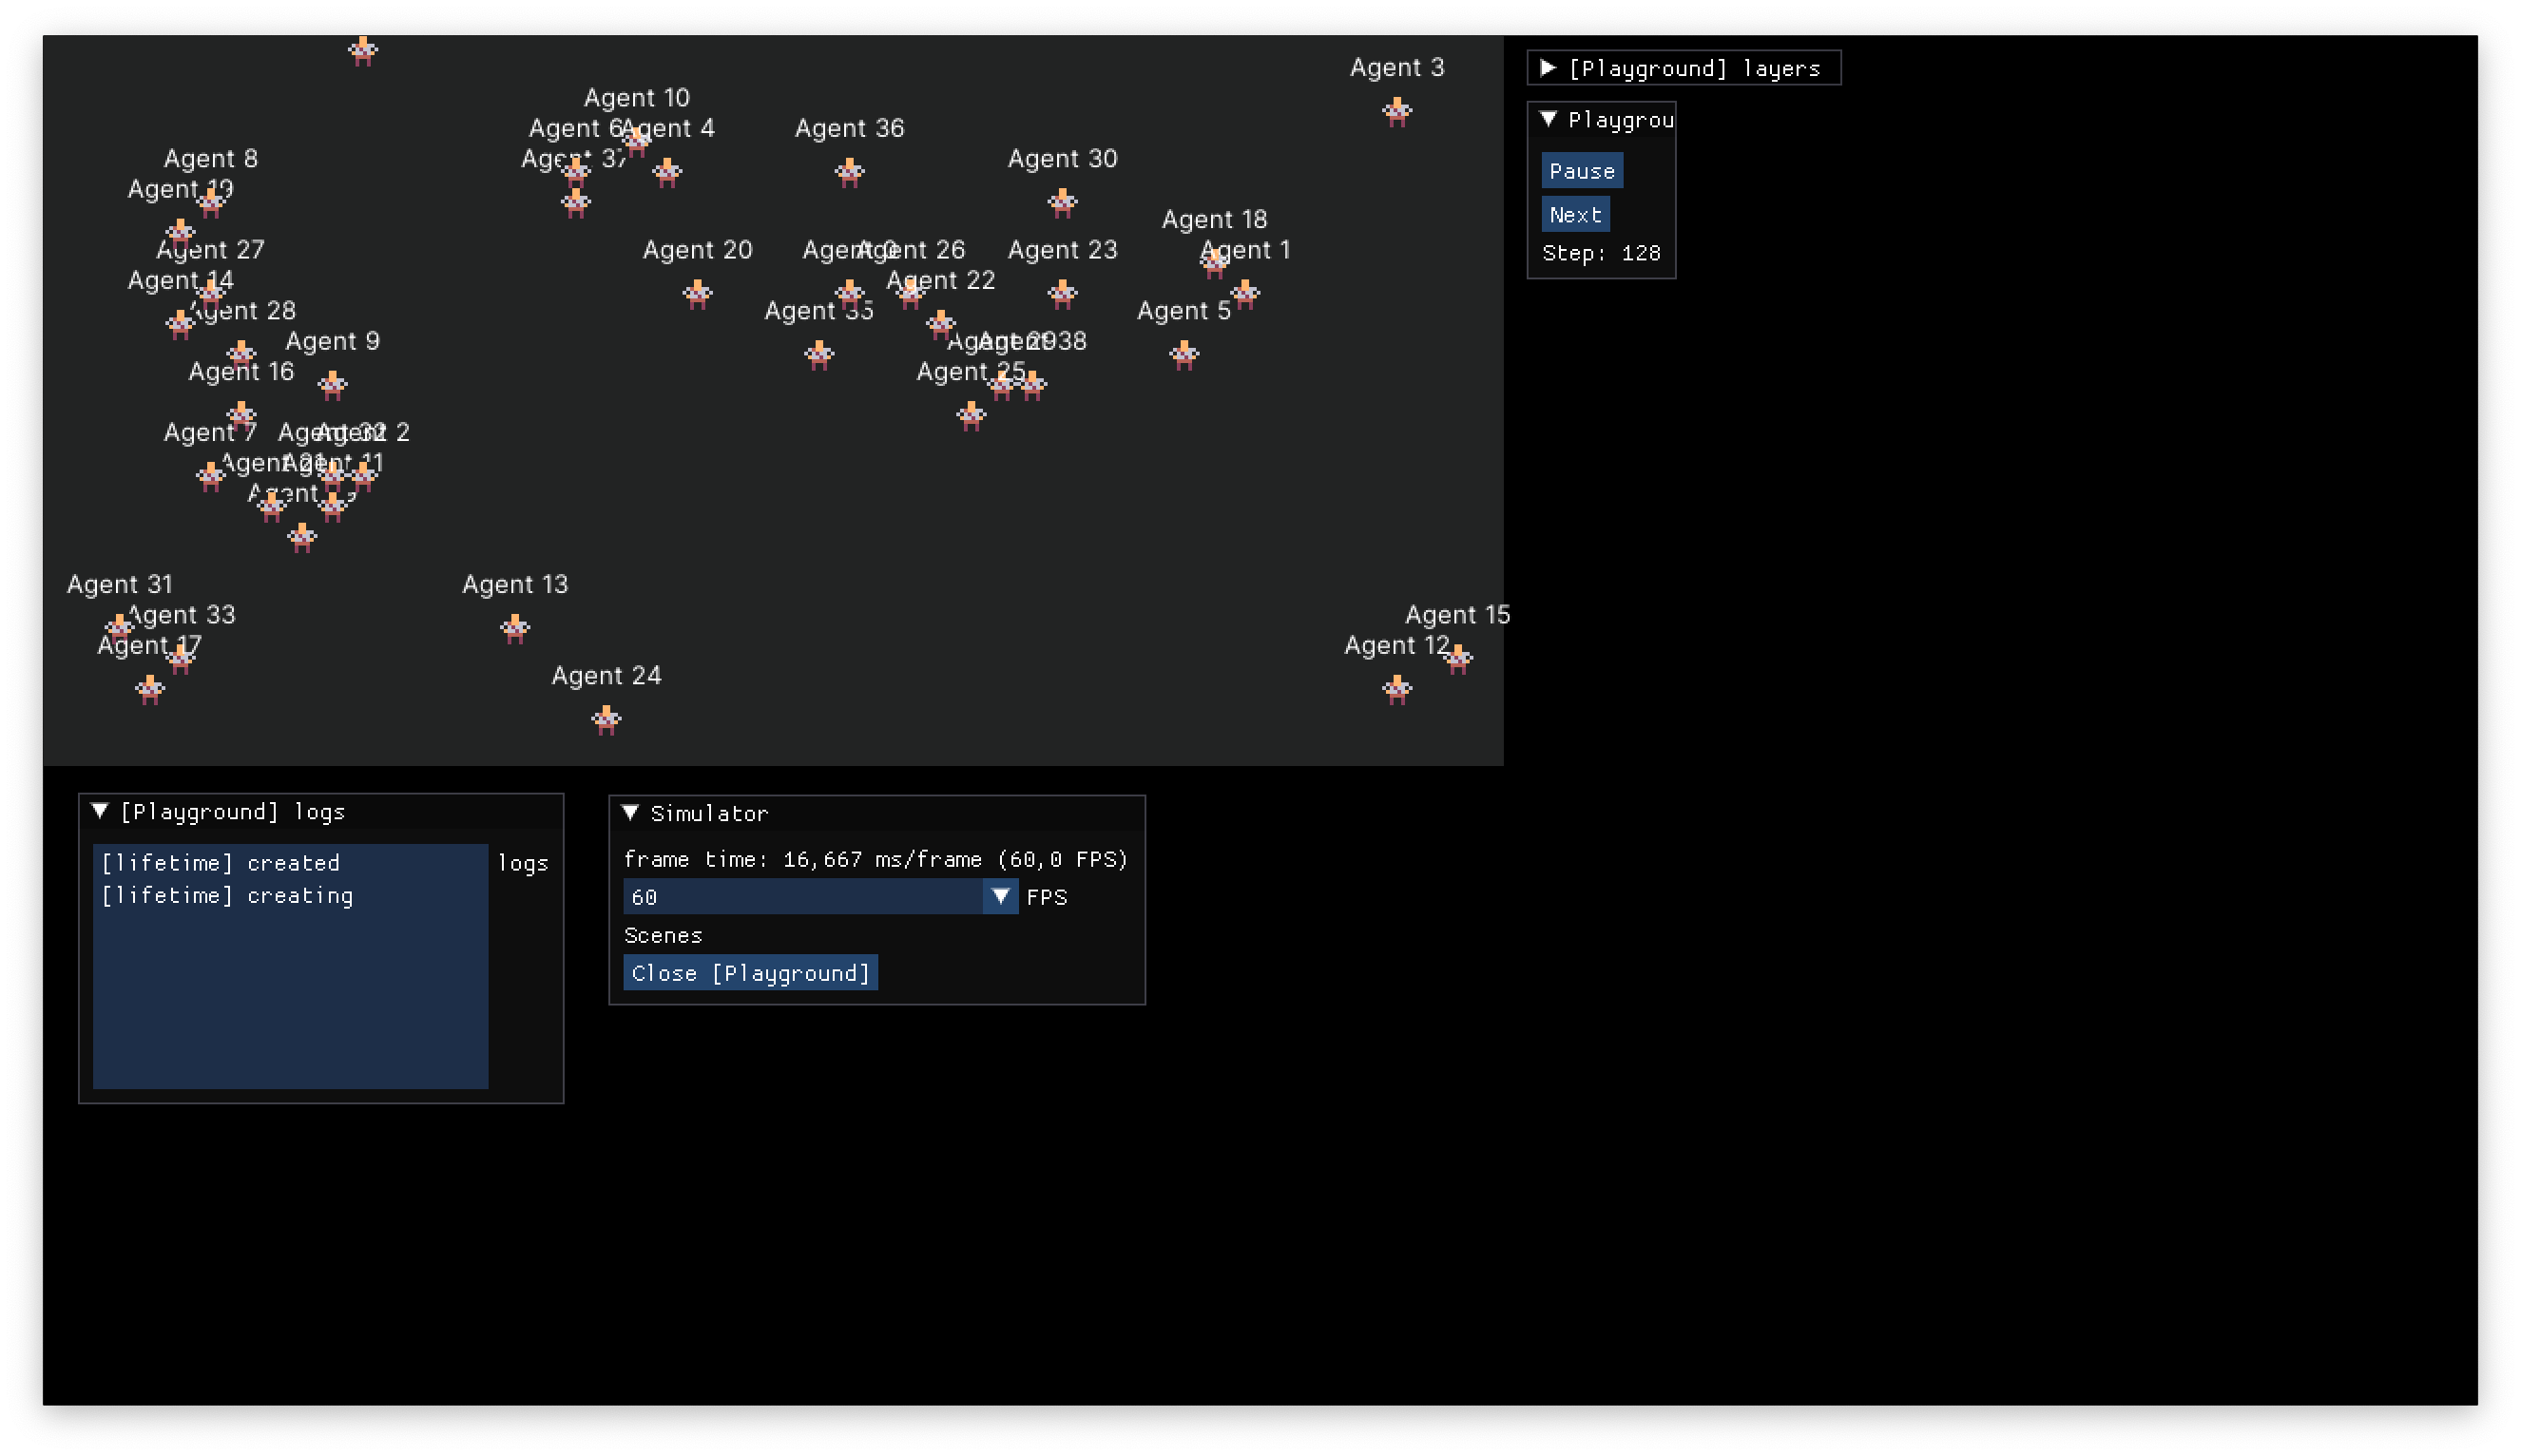
\includegraphics[width=0.3\textwidth]{images/chapter2/sir1/sir_128.png}\label{fig:images/chapter2/sir1/sir_123.png}}

    \caption{Experiment 2} \label{fig:experiment1}
\end{figure}

It is worth noting that because the $\gamma$ parameter was set to zero, no agents could recover from being infected and so the equations were simplified to the following.

\begin{equation} \label{eq:sir1_gamma0}
    \frac{{dS}}{{dt}} = -\frac{{\beta \cdot S \cdot I}}{{N}}
\end{equation}

\begin{equation} \label{eq:sir2_gamma0}
    \frac{{dI}}{{dt}} = \frac{{\beta \cdot S \cdot I}}{{N}}
\end{equation}

\begin{equation} \label{eq:sir3_gamma0}
    \frac{{dR}}{{dt}} = 0
\end{equation}

One can easily see that now:

\begin{equation}
    \frac{{dI}}{{dt}} = -\frac{{dS}}{{dt}}
\end{equation}

\subsection{Experiment 3}

In reality the recovery rate is seldom going to be zero, even in terms of information propagation.
People receive new information every day and even the most interesting news become old and outdated quickly.
In terms of information propagation an agent becoming removed from the simulation signifies that they grew bored of the information or that it became outdated and thus that particular agent is no longer going to participate in spreading it.

% Experiment 3

A rather interesting observation made during testing was that because of the random distribution of agents, when the $\gamma$ parameter was greater than zero, it was often the case that a single individual survived.
Example of this situation is shown on figures \ref{fig:images/chapter2/sir2/sir_1.png}, \ref{fig:images/chapter2/sir2/sir_53.png} and \ref{fig:images/chapter2/sir2/sir_123.png}.
In this particular example the agents' lifetime upon infection became limited to just 24 simulation steps.
The population size change in time is shown on figure \ref{fig:images/chapter2/sir2/sir.png}.

\begin{figure}[H]
    \centering
    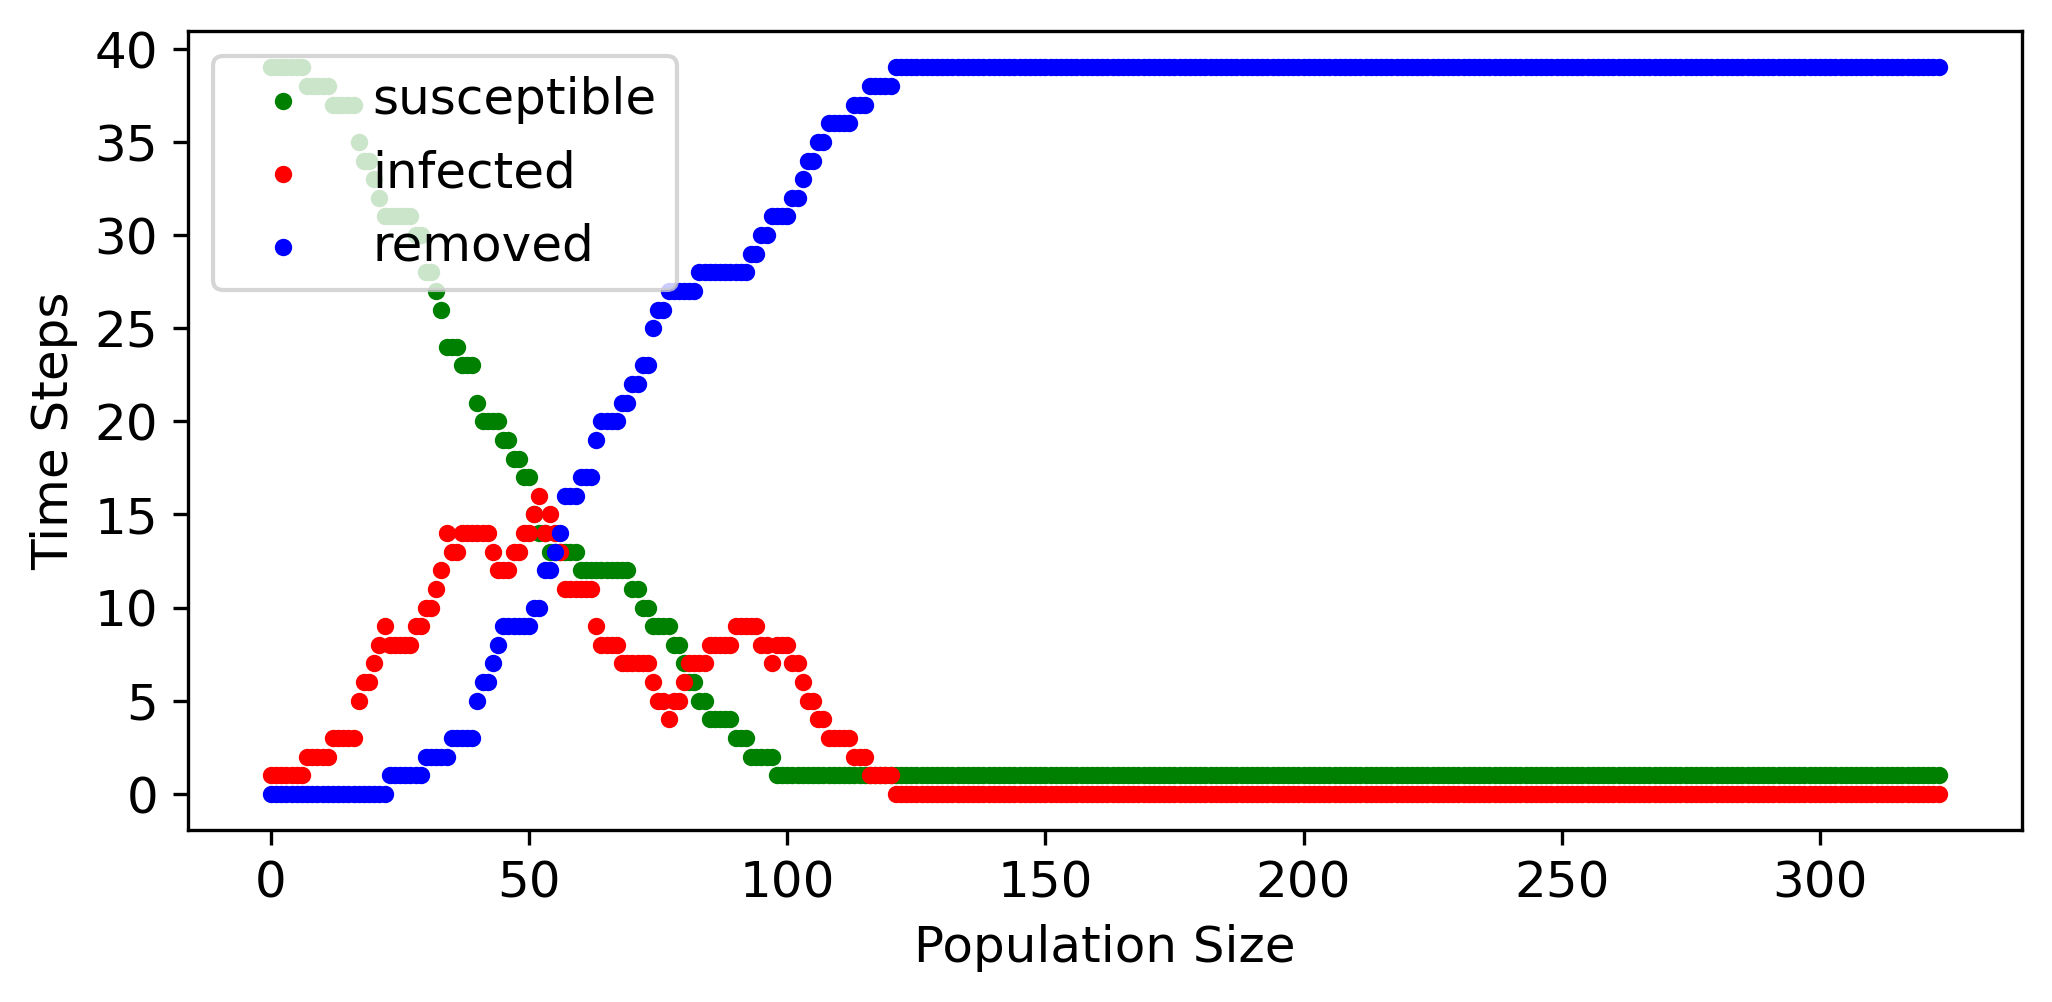
\includegraphics[width=1.0\textwidth]{images/chapter2/sir2/sir.png}
    \caption{Experiment 3 - SIR}\label{fig:images/chapter2/sir2/sir.png}
\end{figure}

\begin{figure}[H]
    \centering
    \subfigure[Step 1]{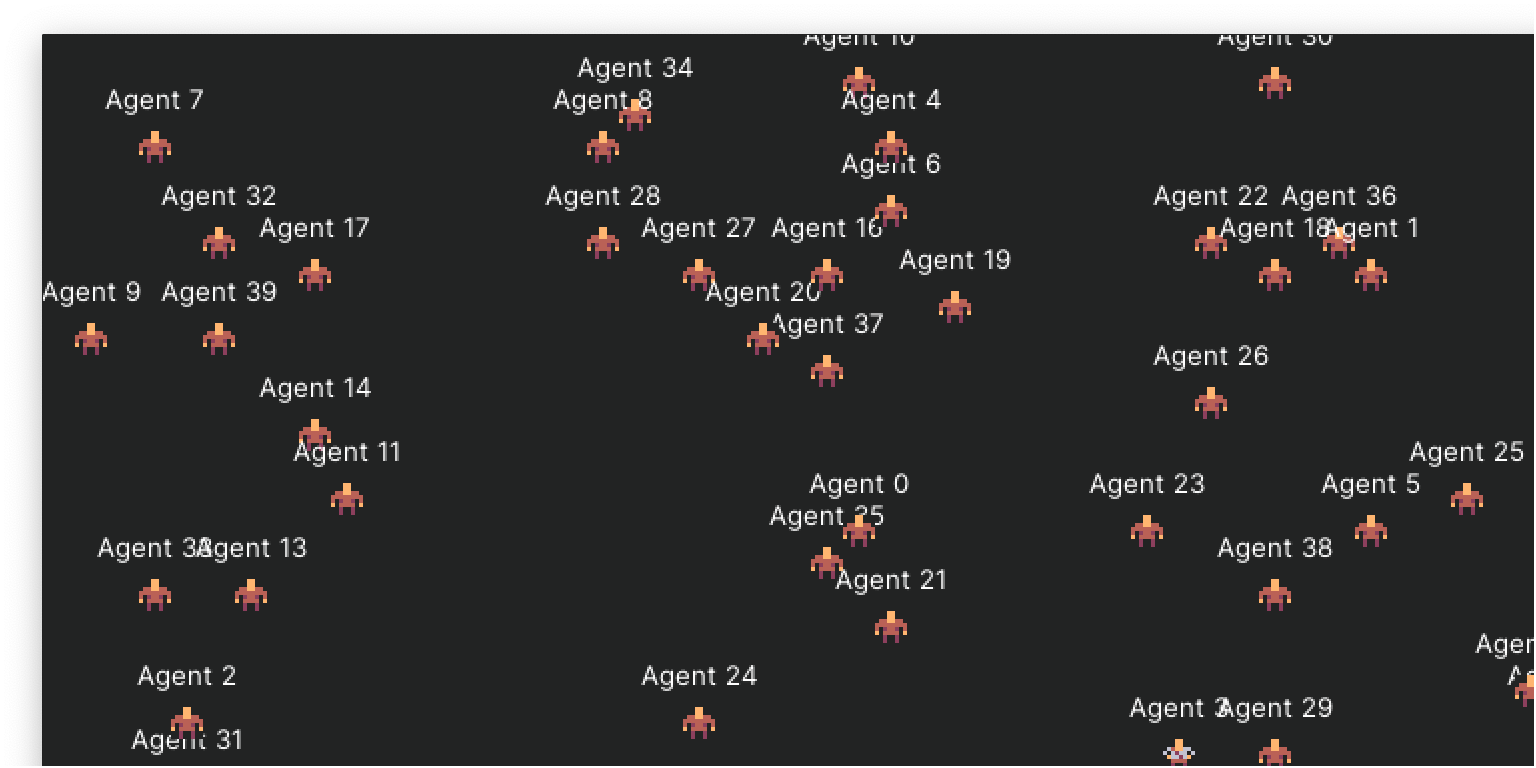
\includegraphics[width=0.3\textwidth]{images/chapter2/sir2/sir_1.png}\label{fig:images/chapter2/sir2/sir_1.png}}
    \hspace*{\fill}
    \subfigure[Step 53]{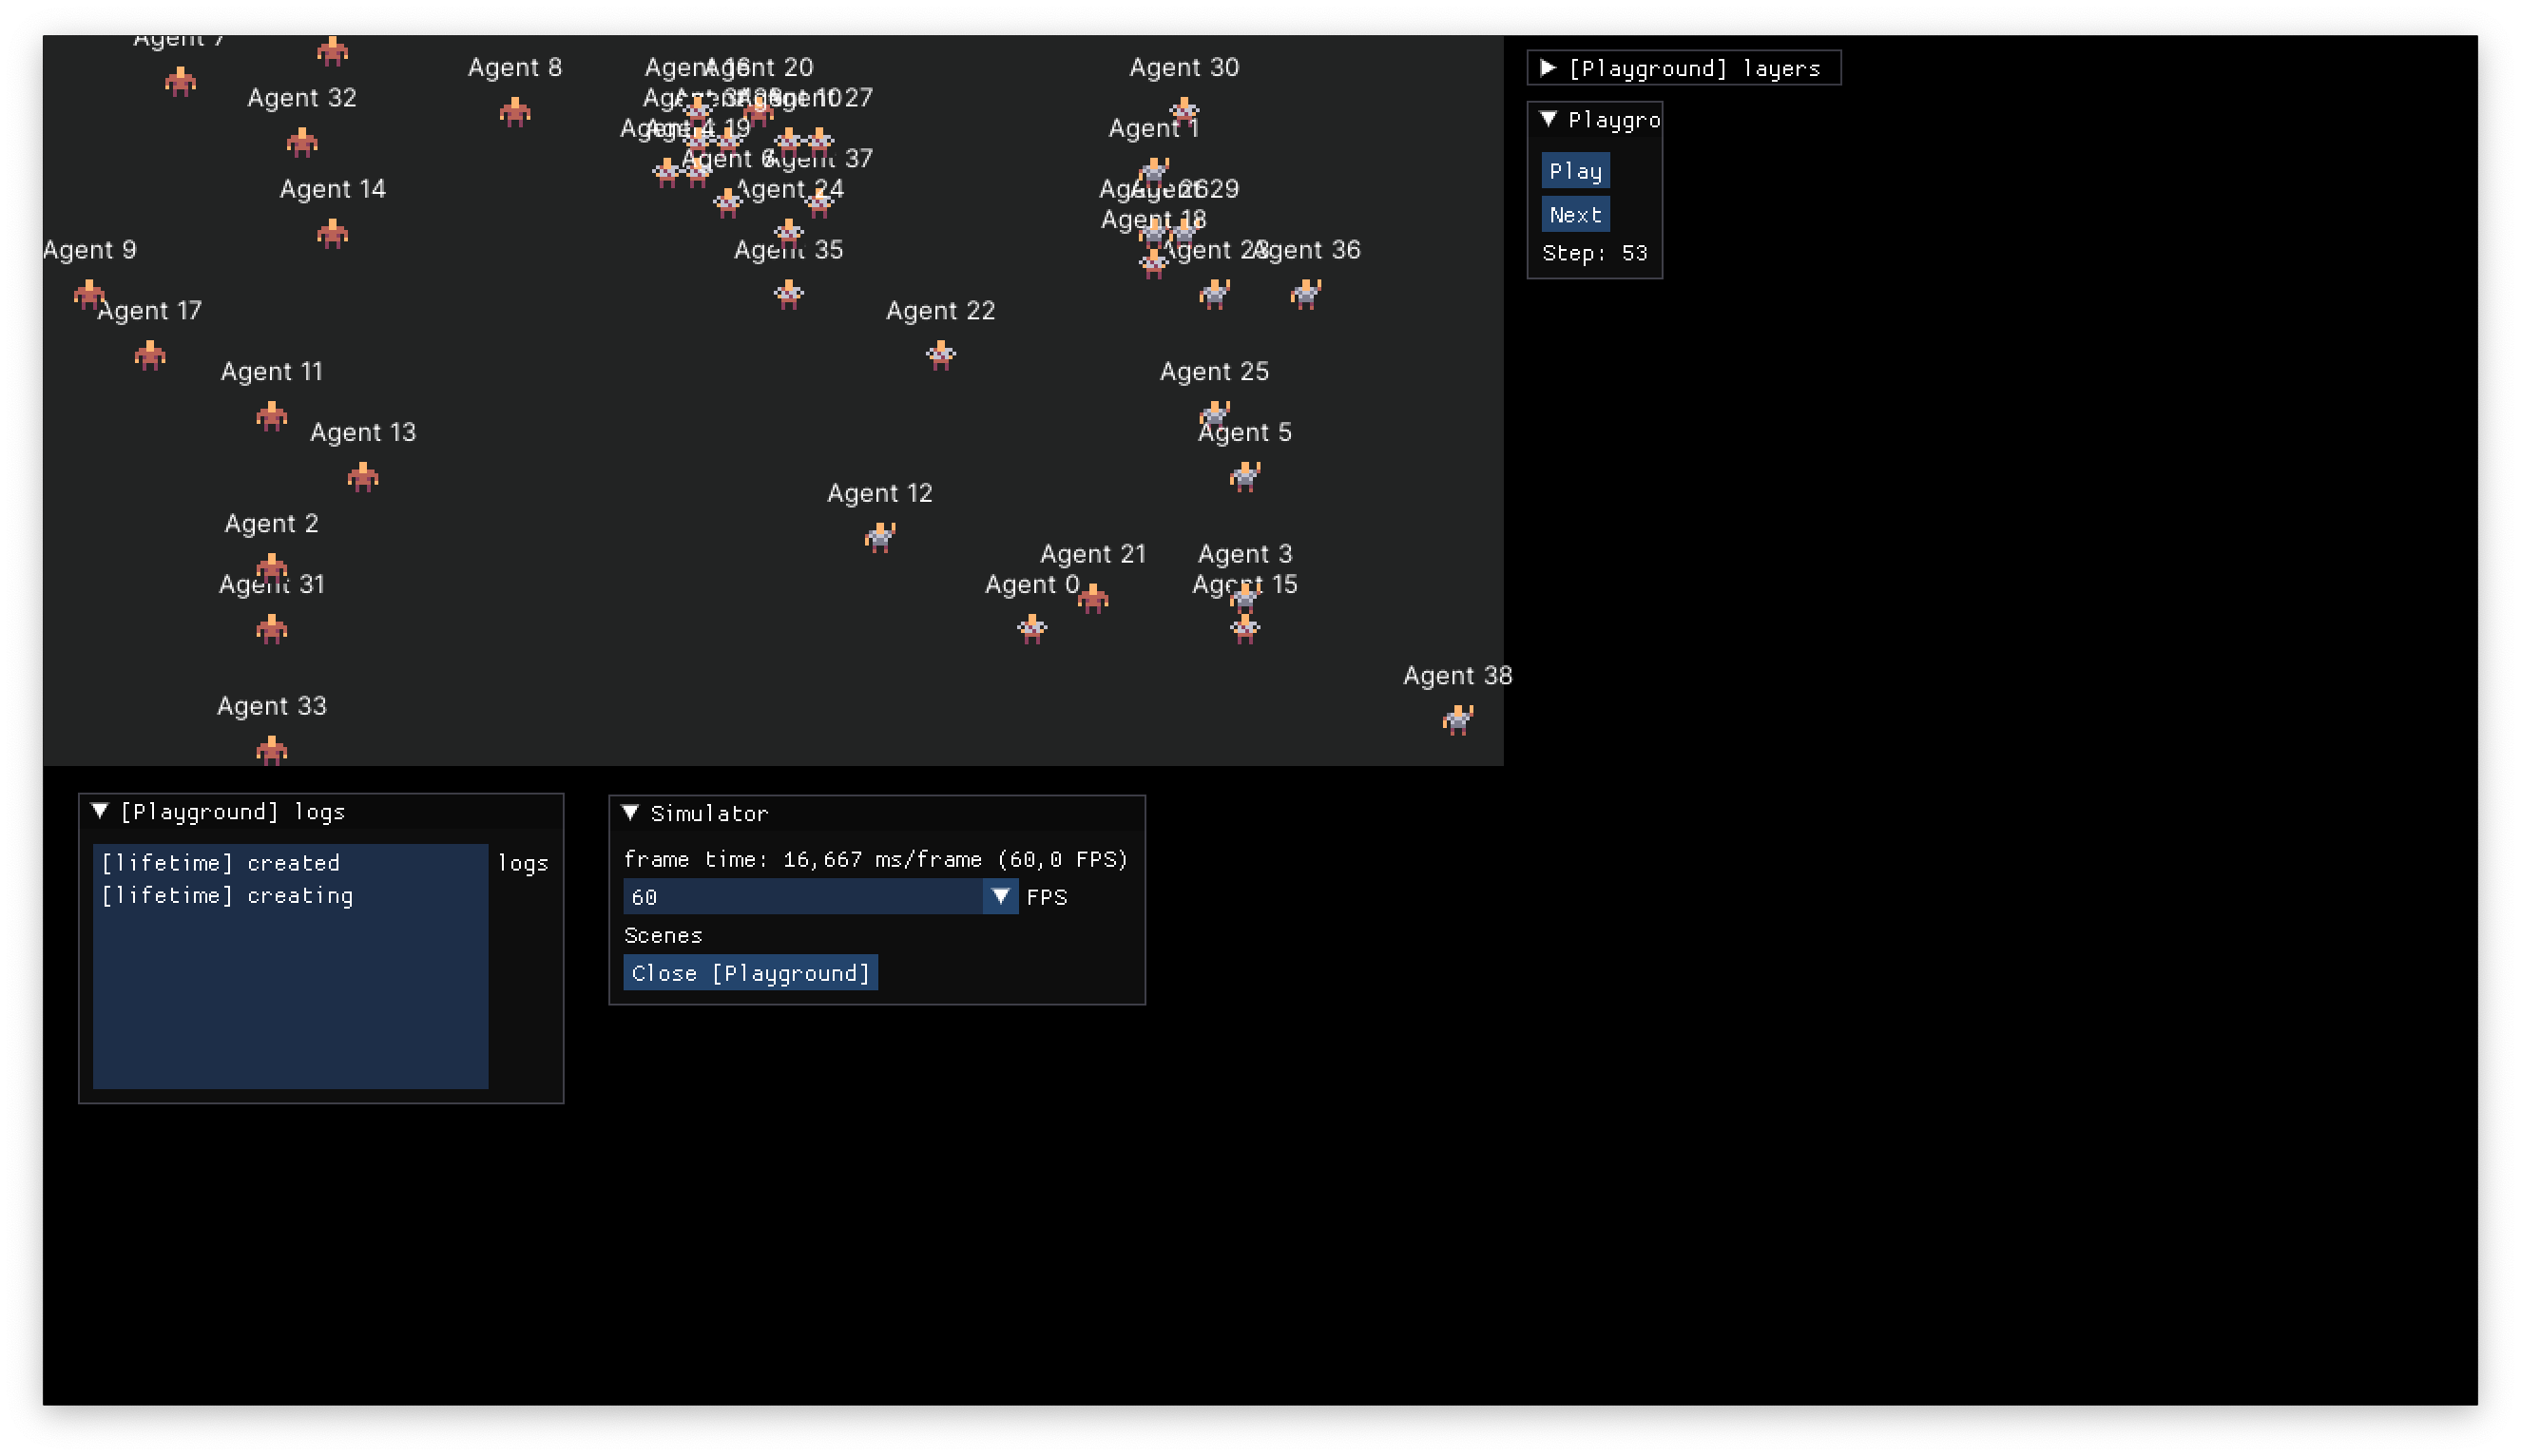
\includegraphics[width=0.3\textwidth]{images/chapter2/sir2/sir_53.png}\label{fig:images/chapter2/sir2/sir_53.png}}
    \hspace*{\fill}
    \subfigure[Step 324]{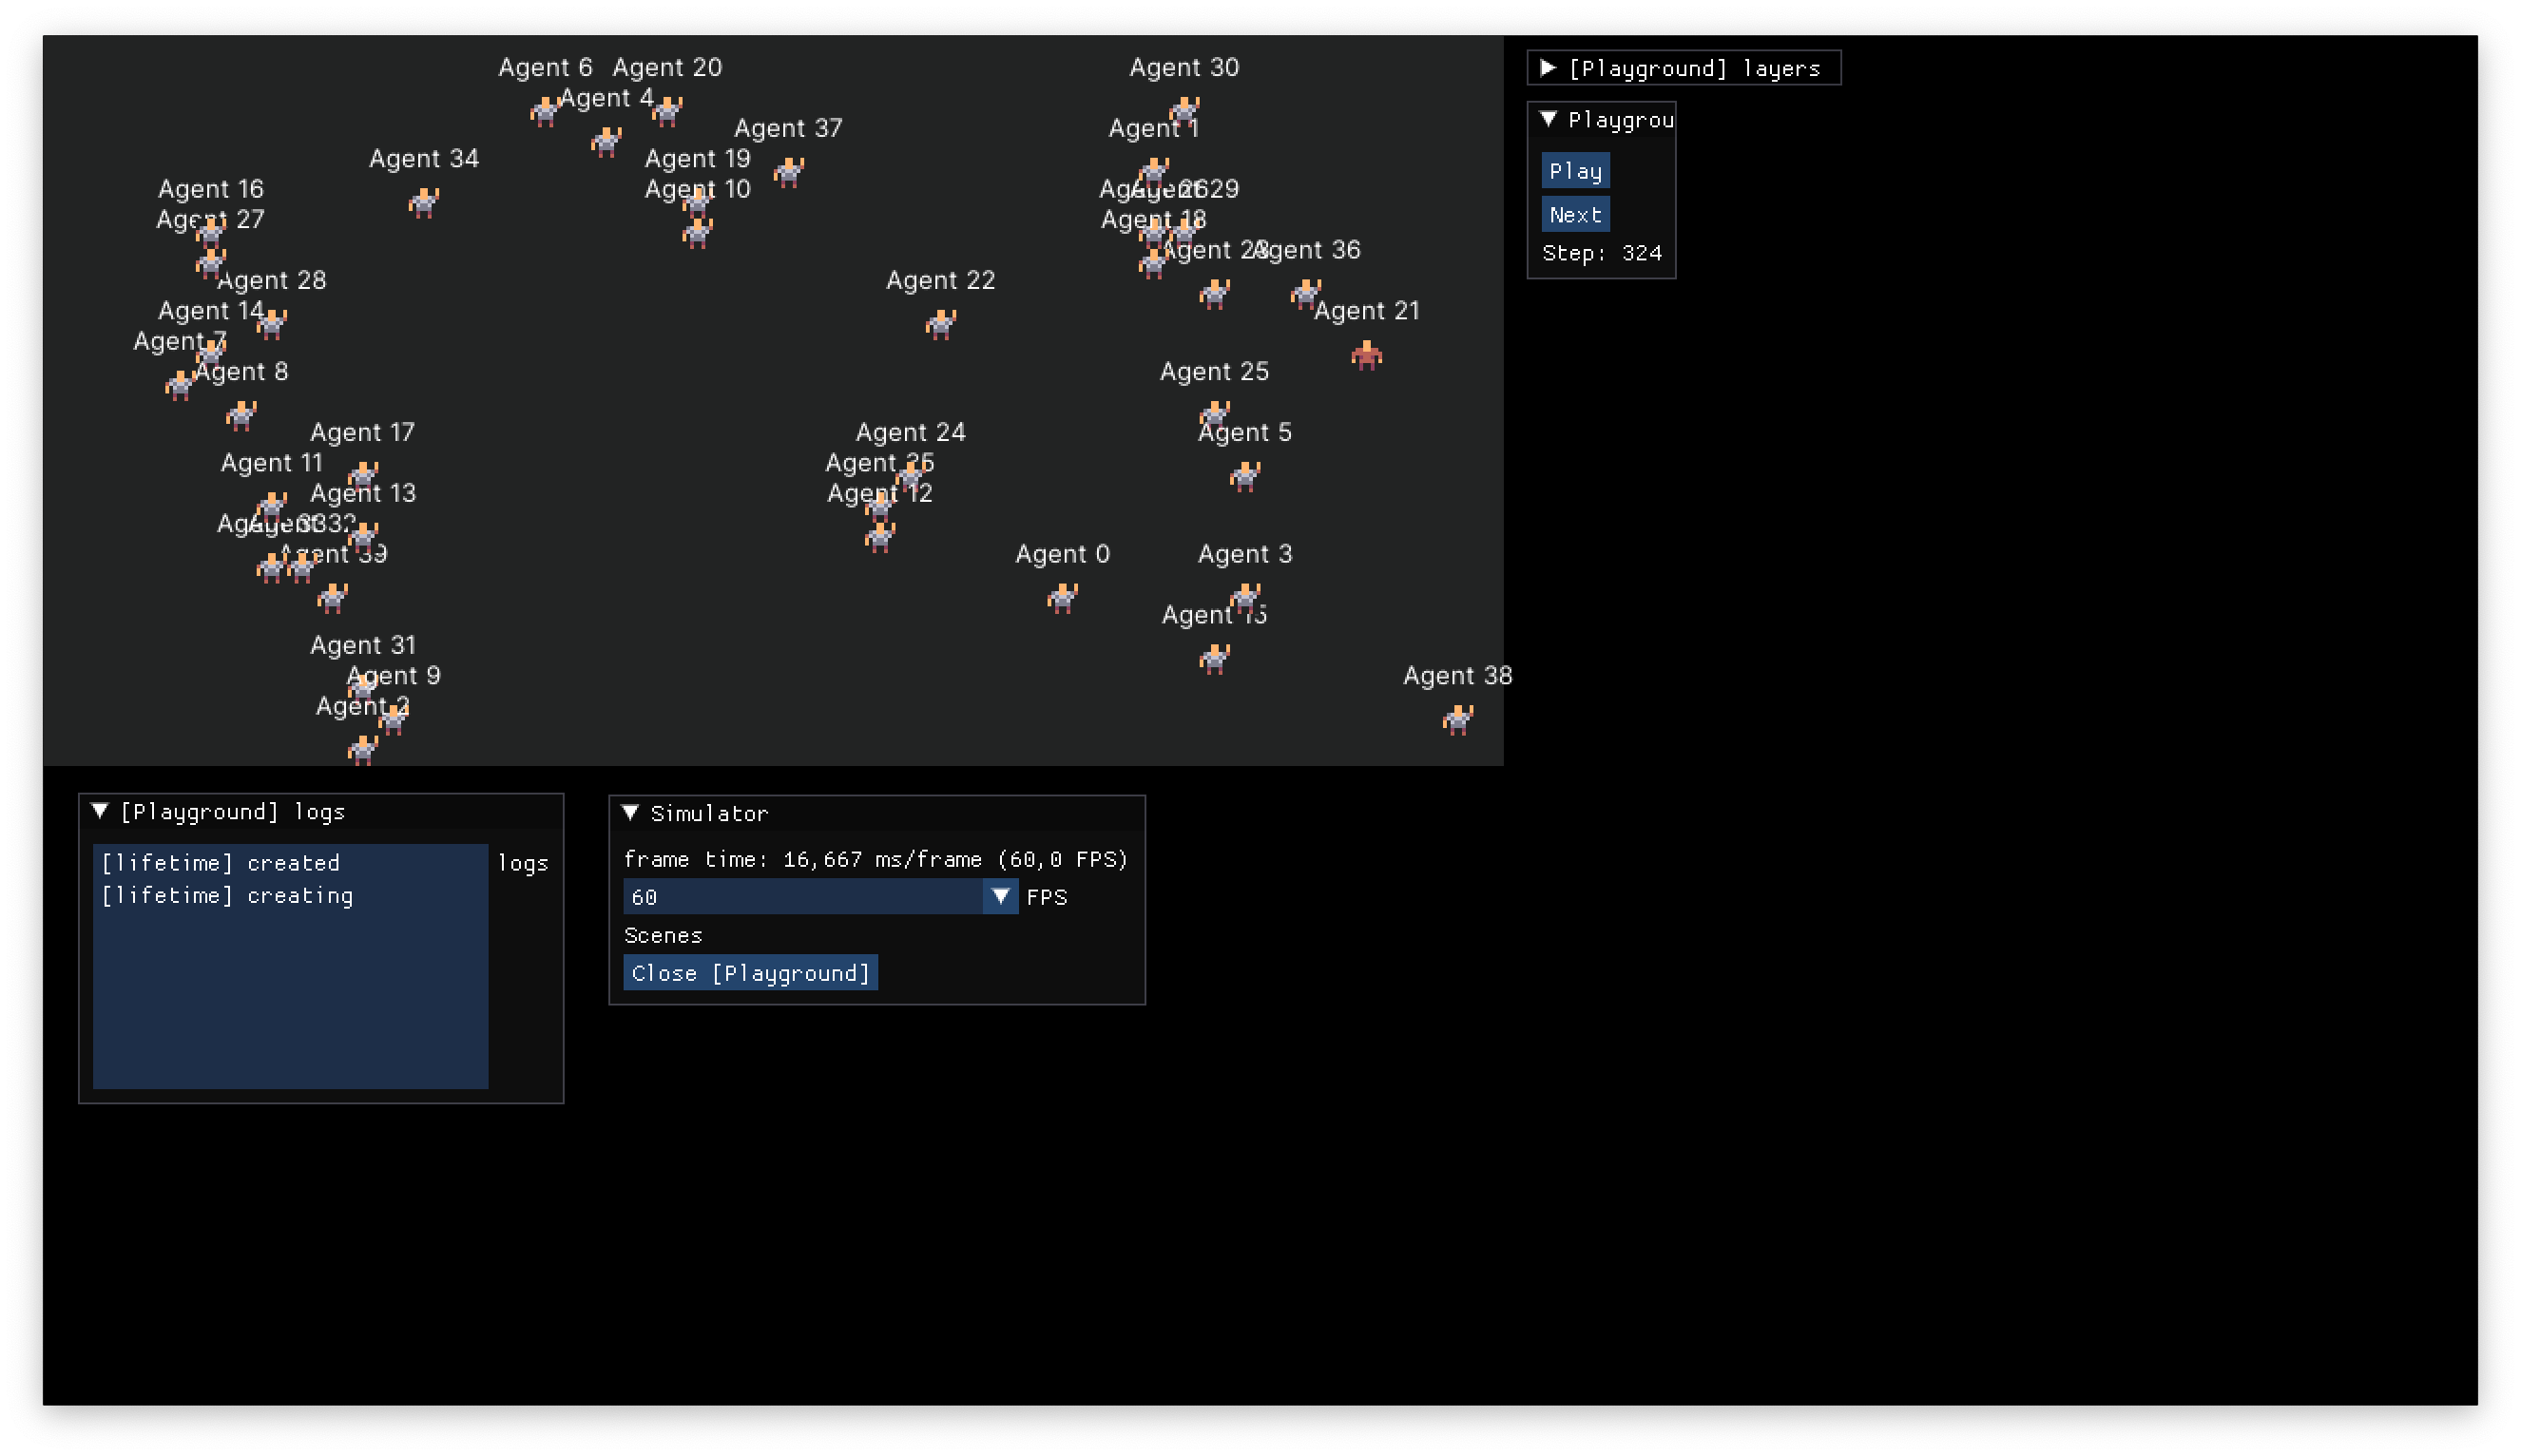
\includegraphics[width=0.3\textwidth]{images/chapter2/sir2/sir_324.png}\label{fig:images/chapter2/sir2/sir_123.png}}

    \caption{Experiment 3} \label{fig:experiment2}
\end{figure}

\subsection{Experiment 4}

Normally the recovery rate $\gamma$ is high enough that a disease does not overwhelm the whole population.
The next experiment shows an example of a simulation where infection rate is balanced with the recovery rate such that the number of infected individuals is on roughly the same level.

% Experiment 4

\begin{figure}[H]
    \centering
    \subfigure[Experiment]{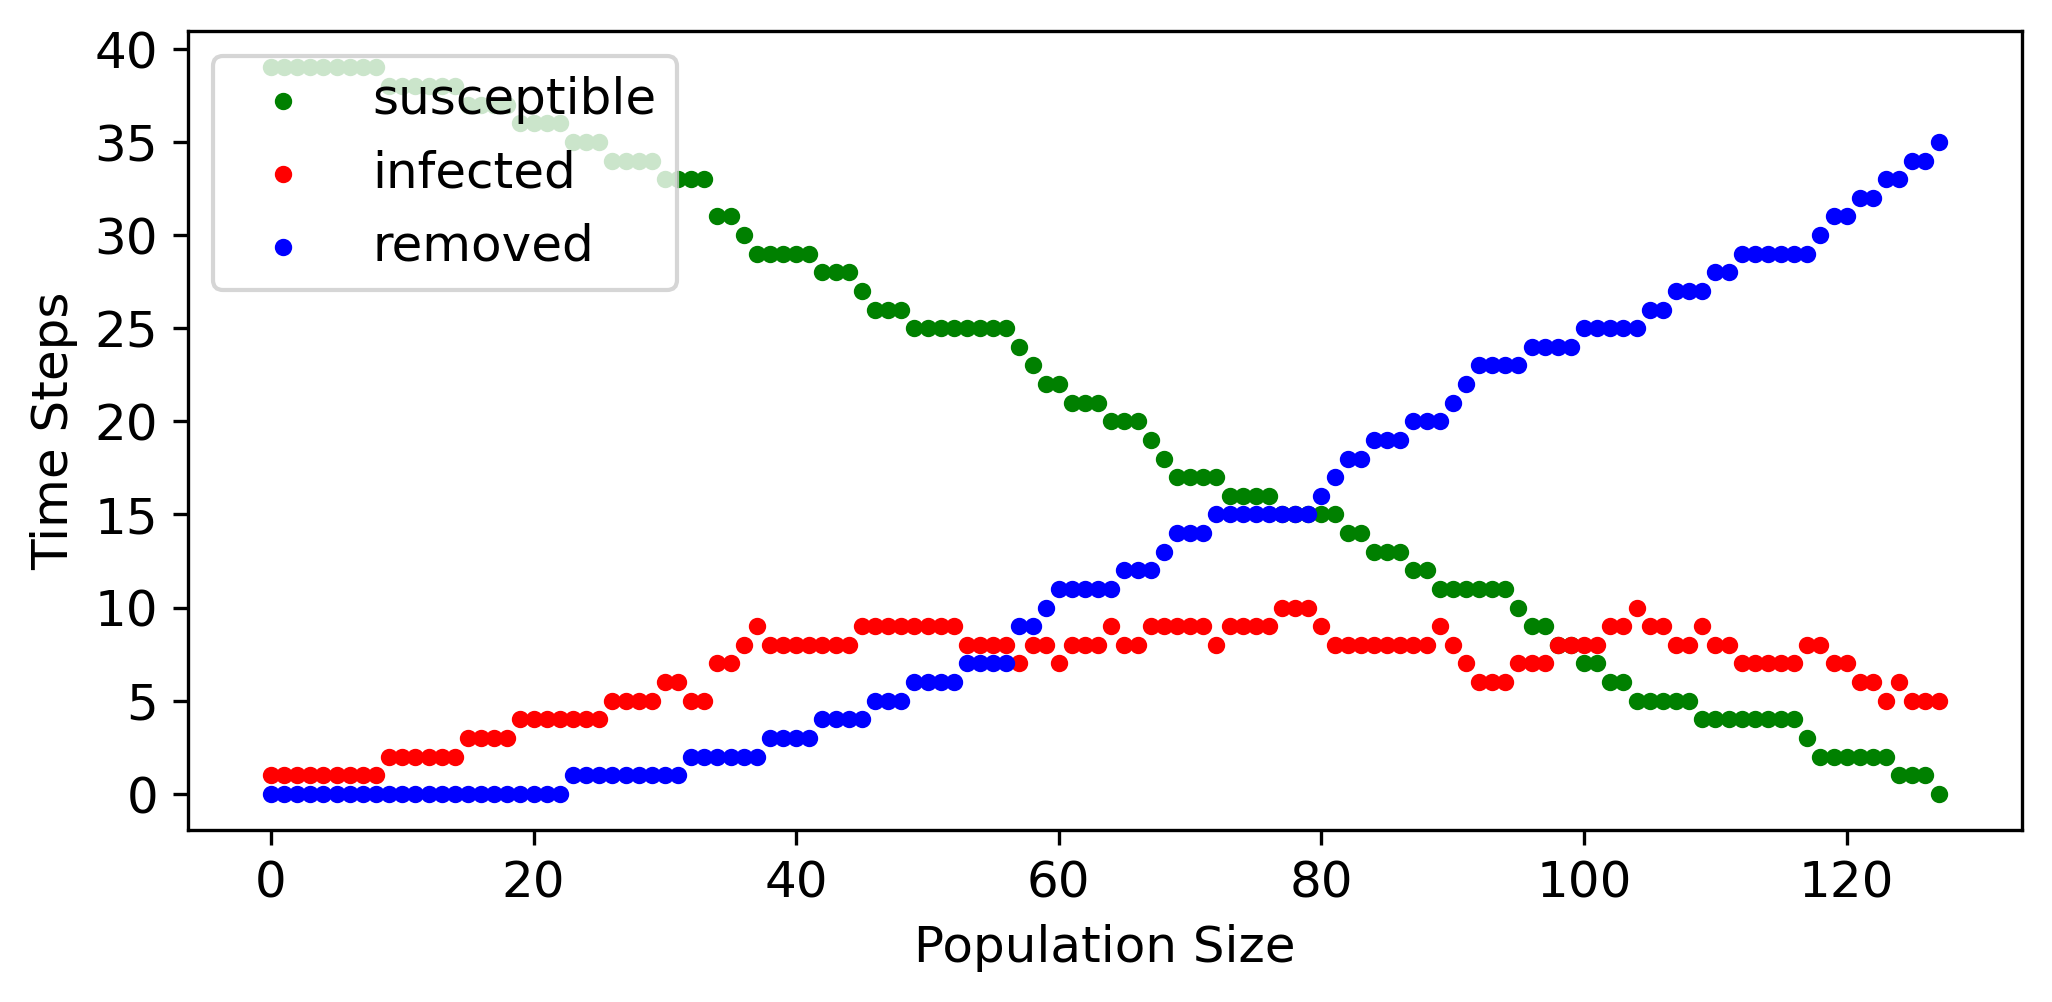
\includegraphics[width=0.48\textwidth]{images/chapter2/sir3/sir.png}\label{fig:images/chapter2/sir3/sir.png}}
    \hspace*{\fill}
    \subfigure[$\beta = 0.03, \gamma = 0.01, N = 40$]{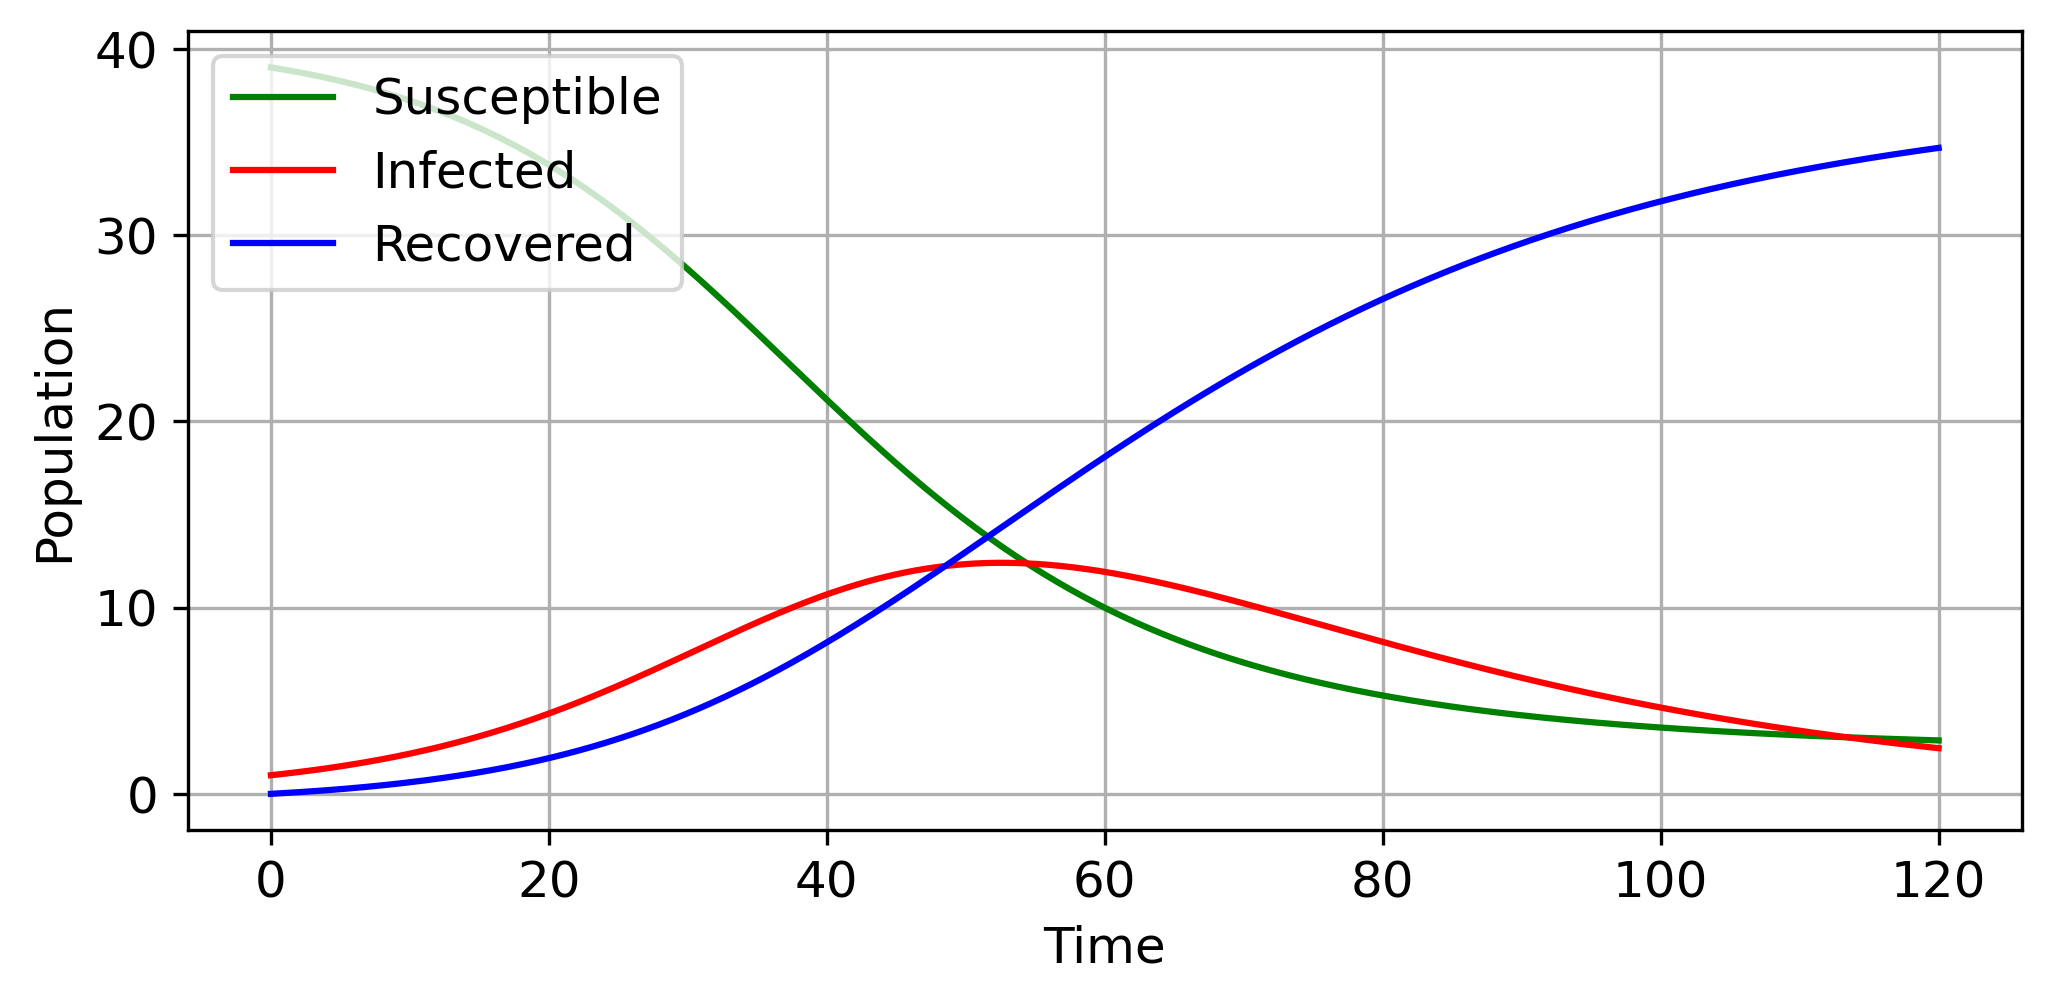
\includegraphics[width=0.48\textwidth]{images/chapter2/sir_ref/sir_2.png}\label{fig:images/chapter2/sir_ref/sir_2.png}}
    \caption{Experiment 4 - SIR vs Experiment} \label{fig:experiment4-diagrams}
\end{figure}

Figure \ref{fig:images/chapter2/sir3/sir.png} illustrates that the level of infection remains somewhat constant for the whole duration of the simulation.
It correlates with the SIR model parameters $\beta = 0.03, \gamma = 0.01, N = 40$ as shown on figure \ref{fig:images/chapter2/sir_ref/sir_2.png}.
Figures \ref{fig:images/chapter2/sir3/sir_1.png}, \ref{fig:images/chapter2/sir3/sir_79.png} and \ref{fig:images/chapter2/sir3/sir_128.png} show the progression of the simulation up until the last susceptible individual changes state.

\begin{figure}[H]
    \centering
    \subfigure[Step 1]{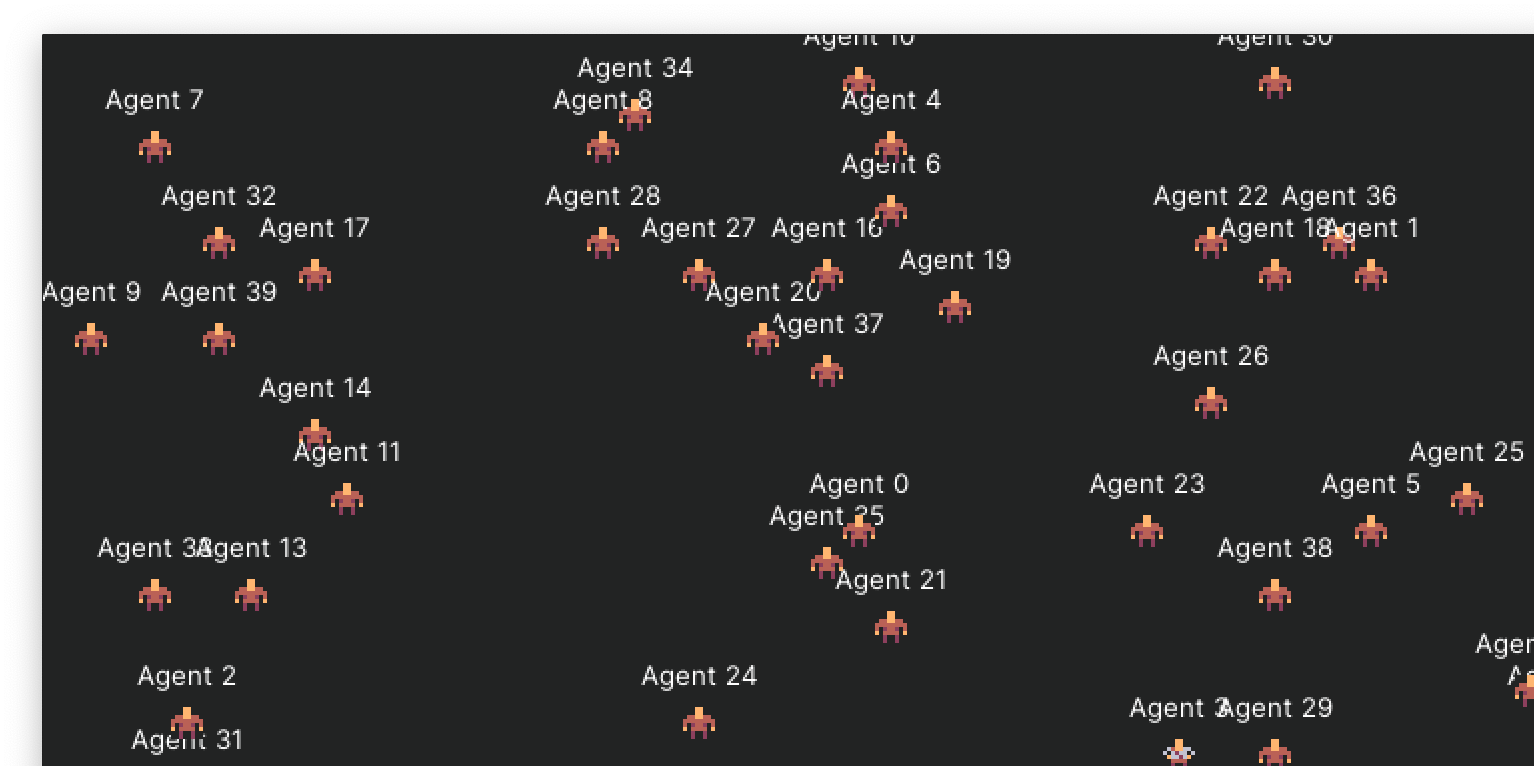
\includegraphics[width=0.3\textwidth]{images/chapter2/sir3/sir_1.png}\label{fig:images/chapter2/sir3/sir_1.png}}
    \hspace*{\fill}
    \subfigure[Step 79]{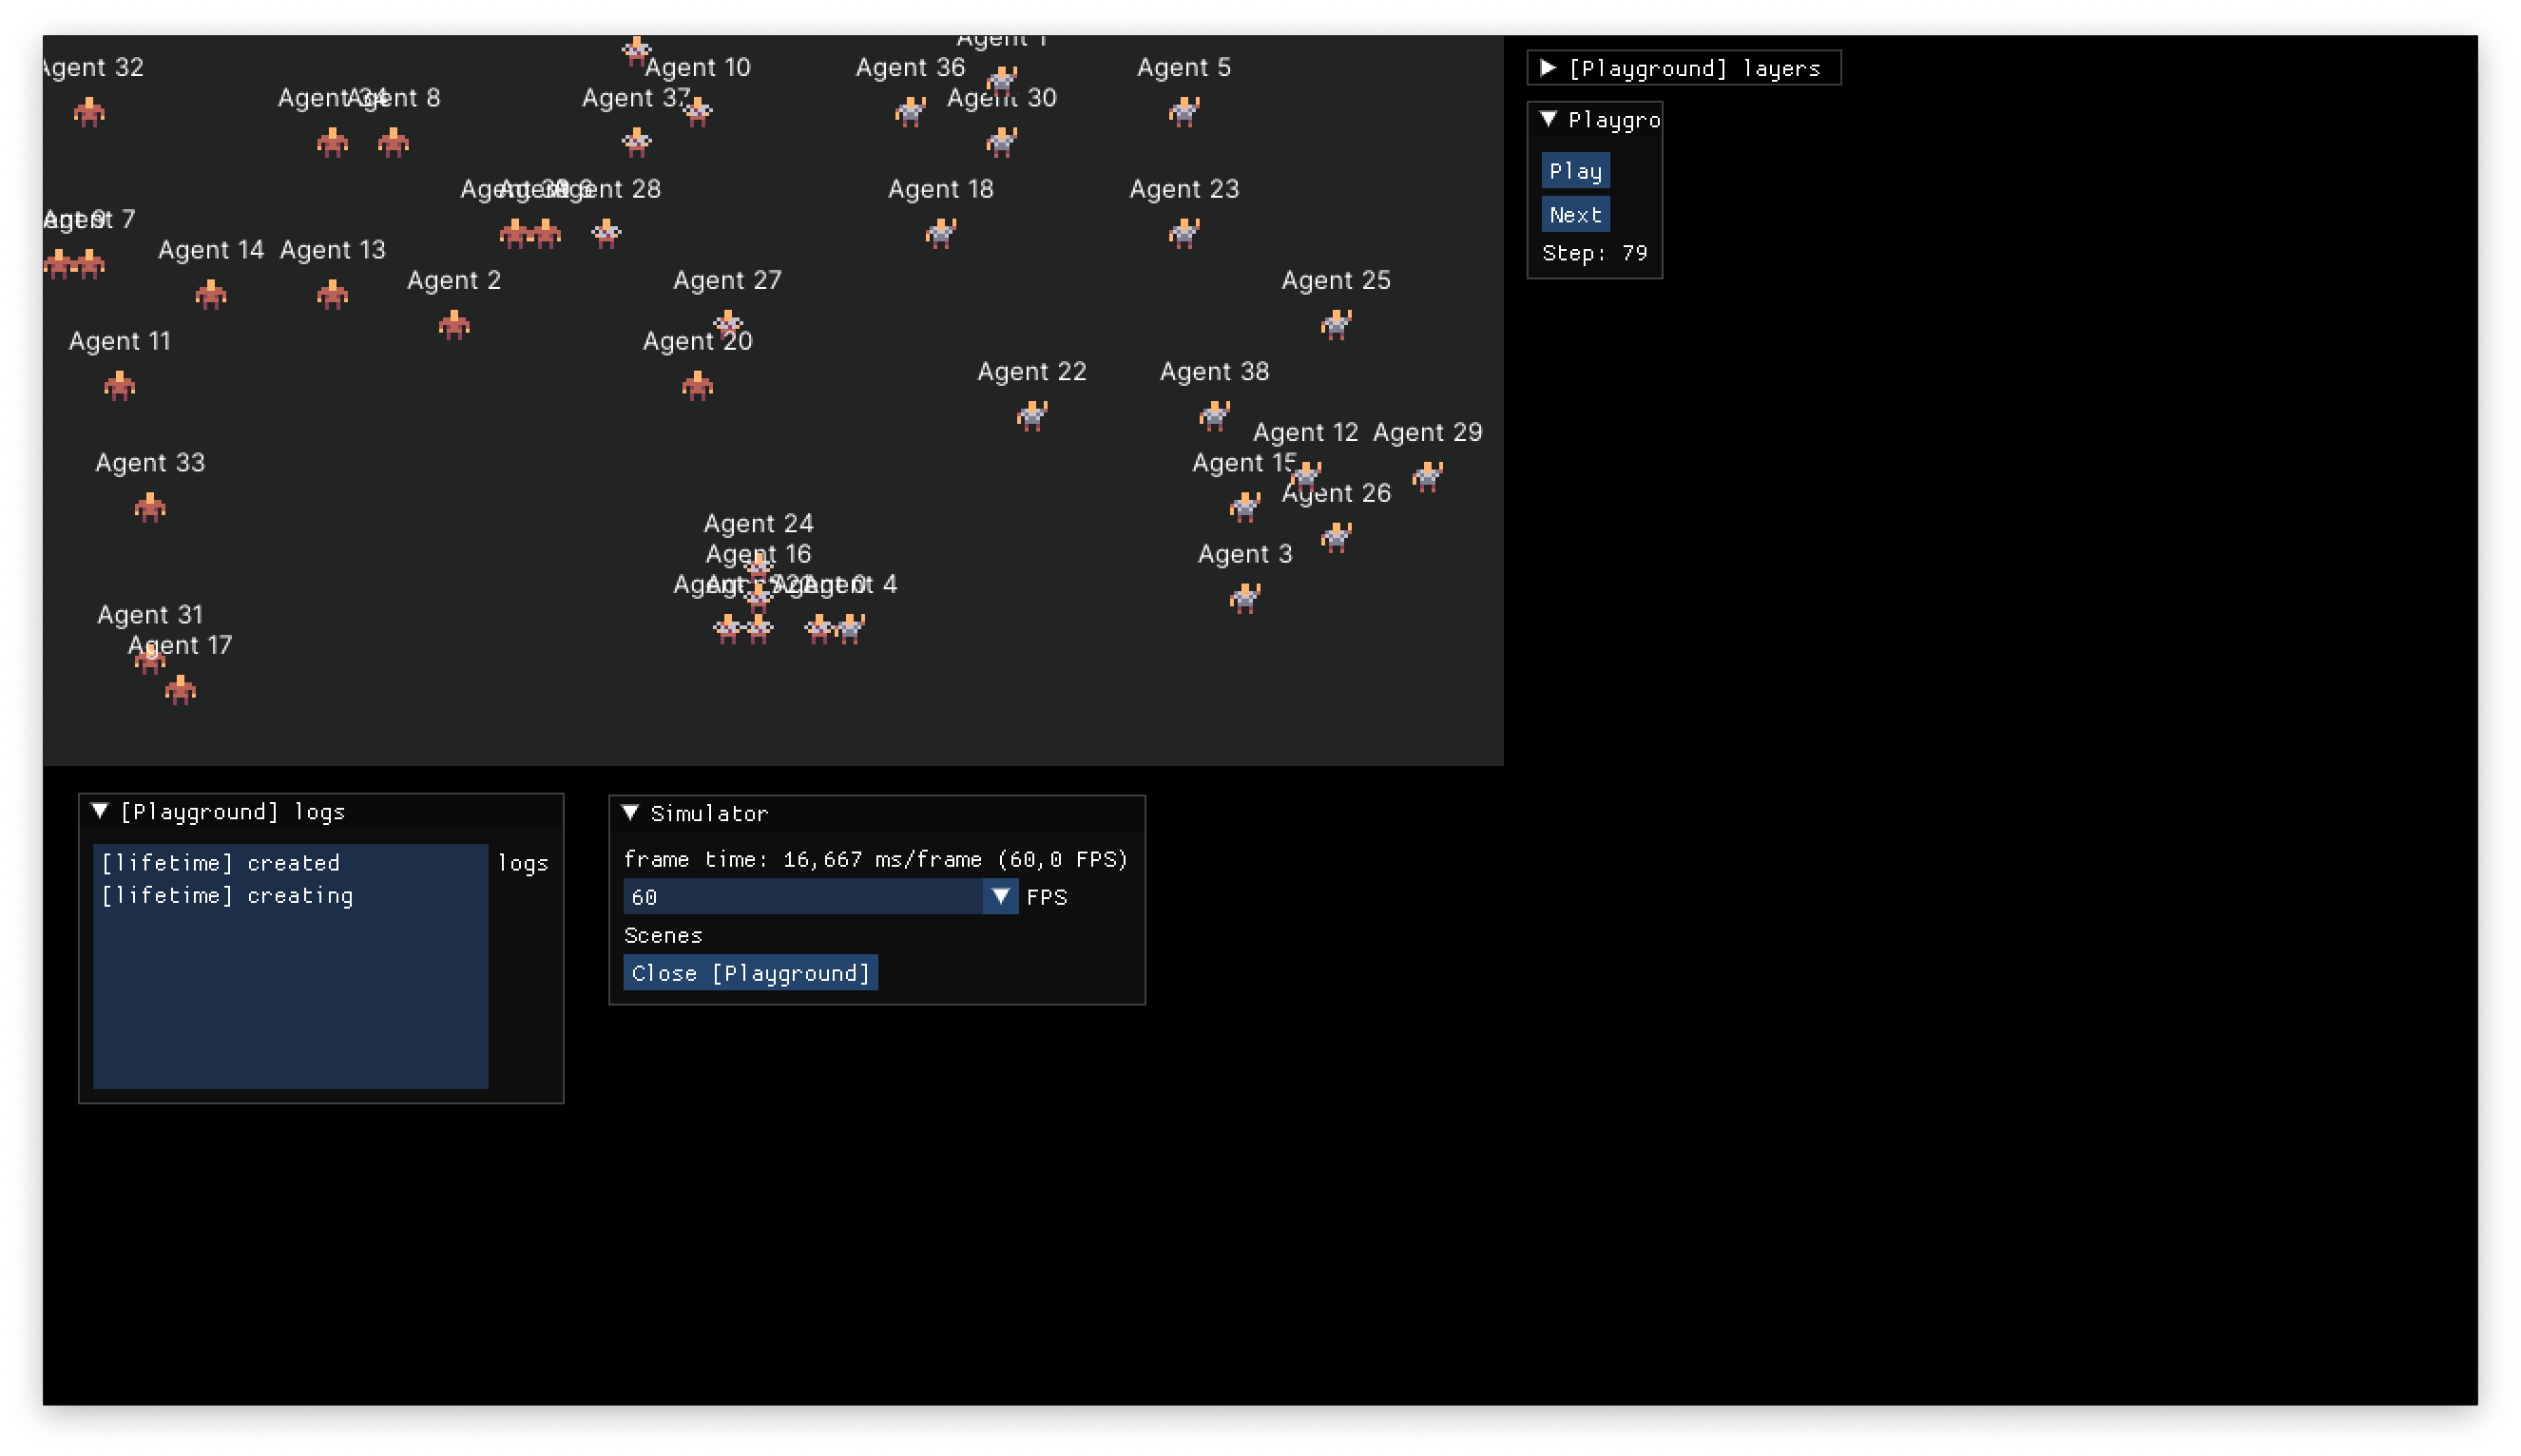
\includegraphics[width=0.3\textwidth]{images/chapter2/sir3/sir_79.png}\label{fig:images/chapter2/sir3/sir_79.png}}
    \hspace*{\fill}
    \subfigure[Step 128]{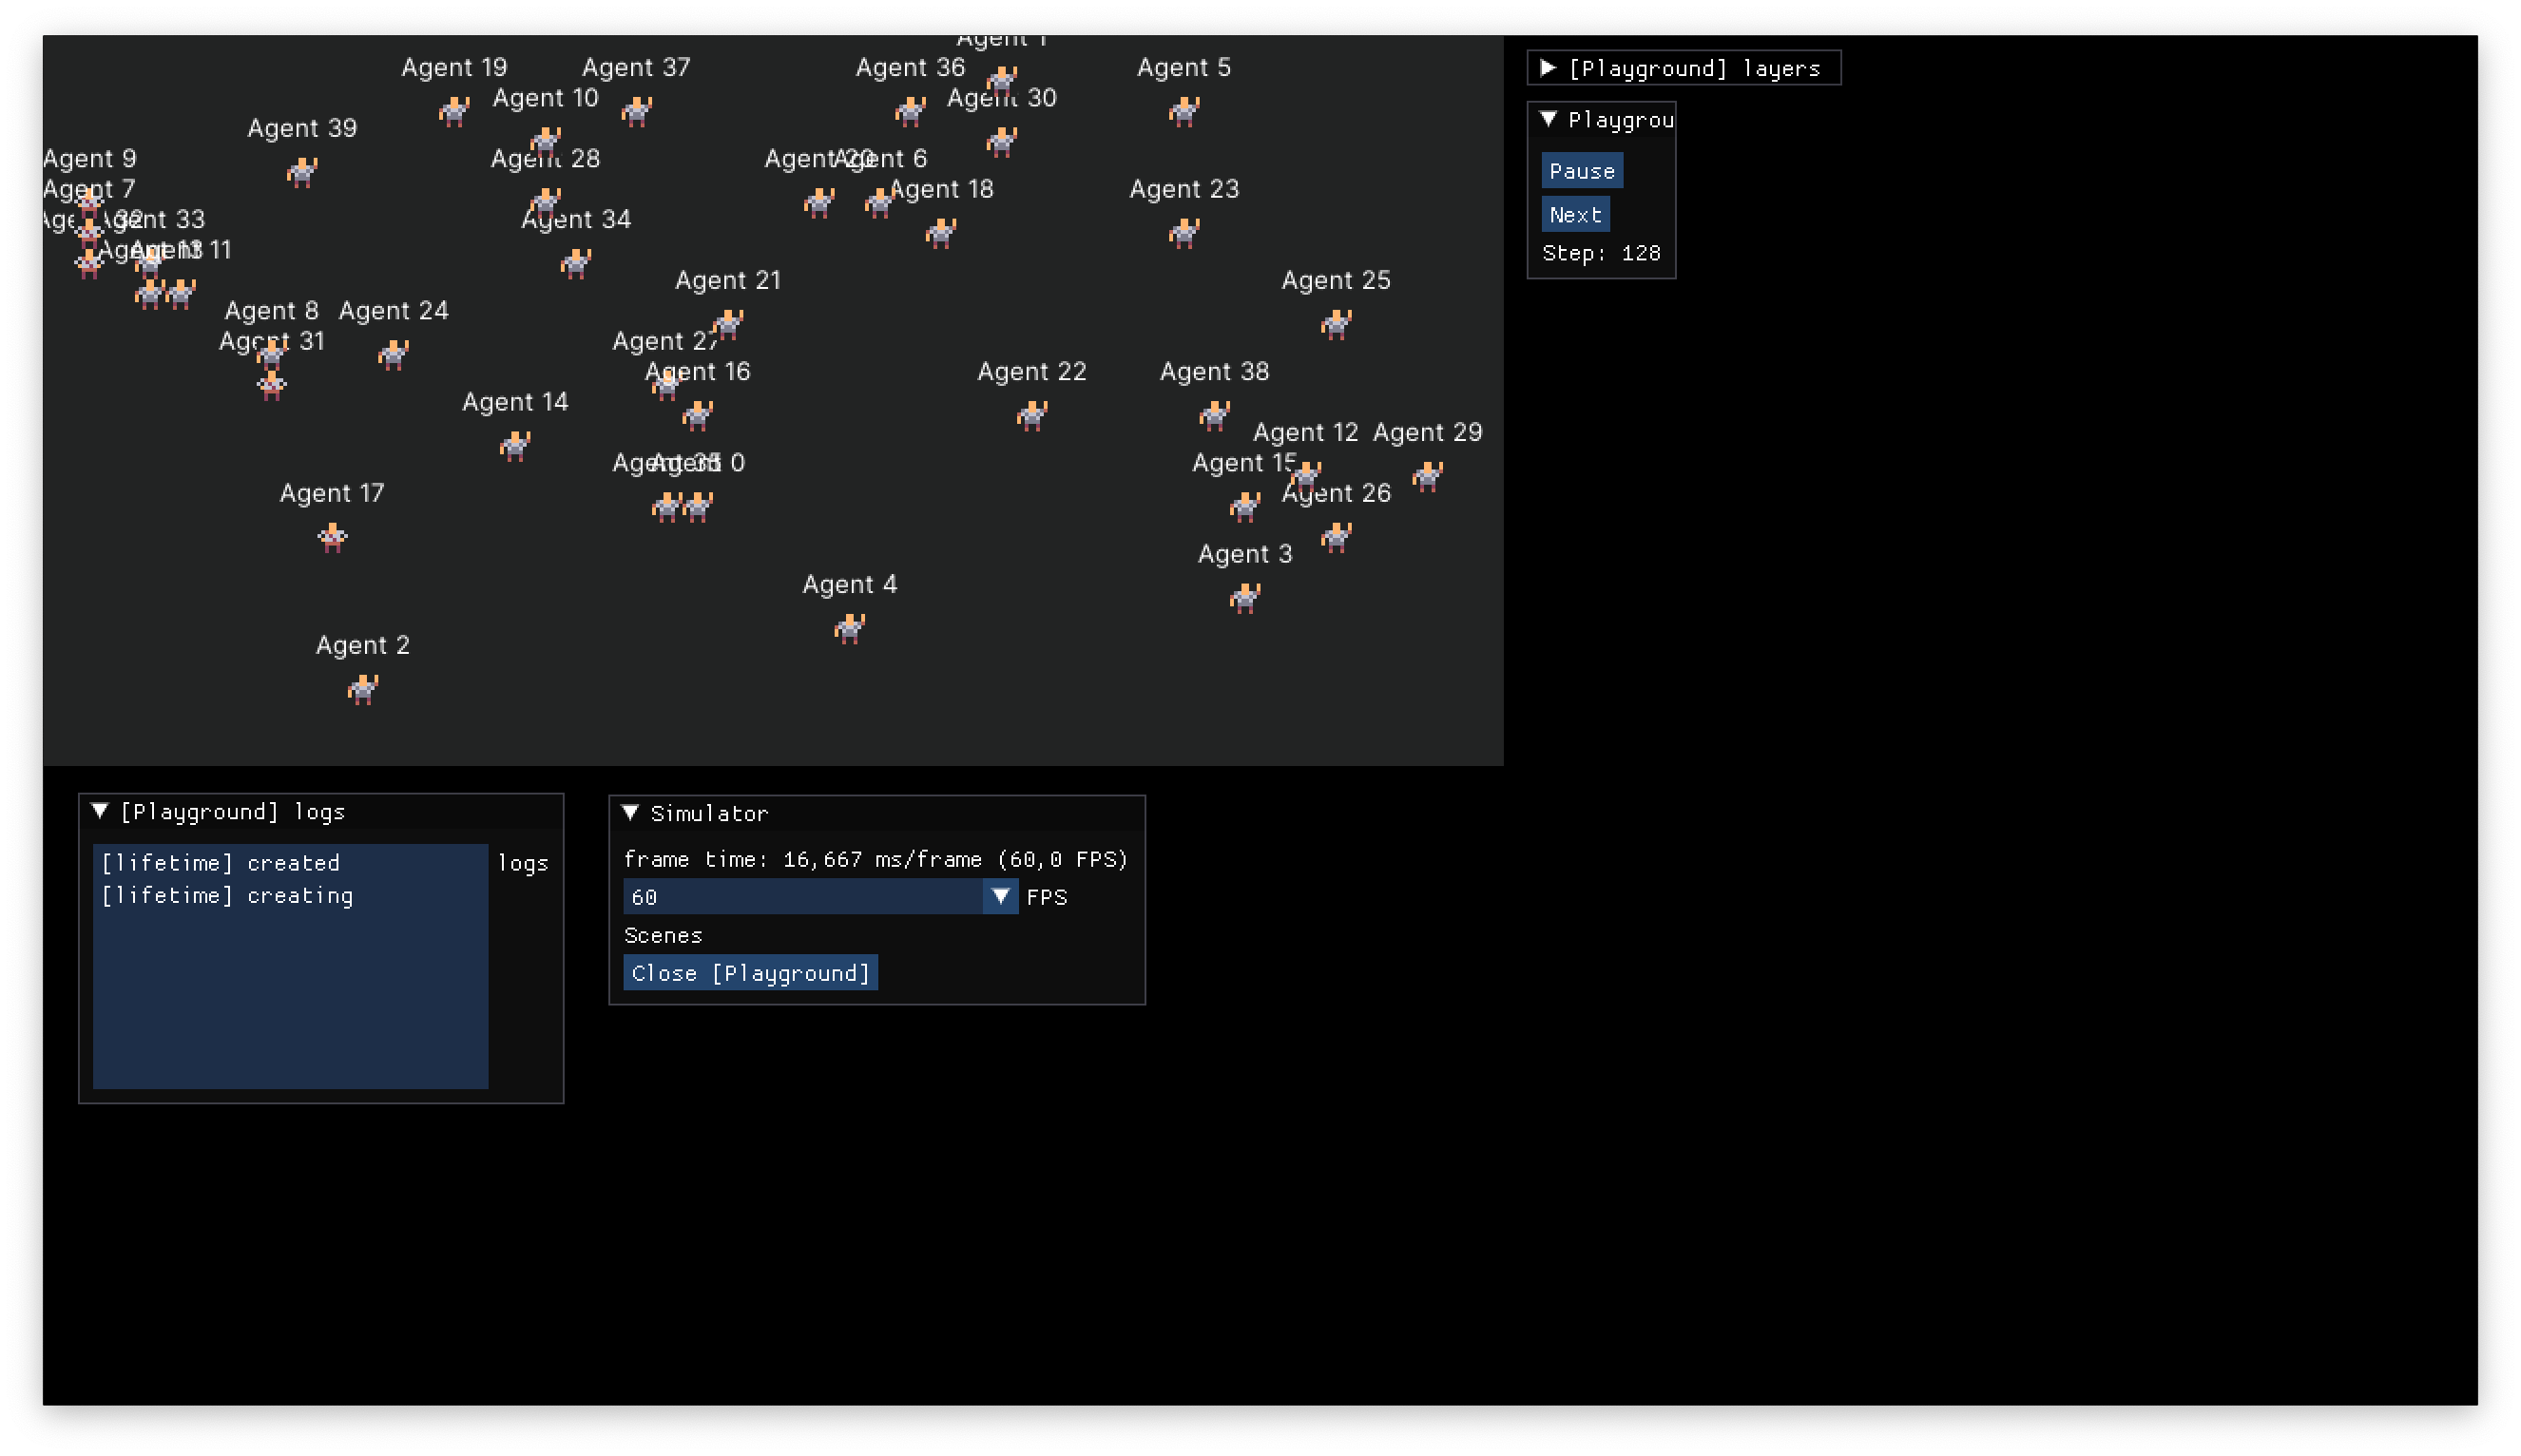
\includegraphics[width=0.3\textwidth]{images/chapter2/sir3/sir_128.png}\label{fig:images/chapter2/sir3/sir_128.png}}

    \caption{Experiment 4} \label{fig:experiment3}
\end{figure}

\subsection{Conclusions}

The experiments have shown that a multi-agent system implemented using the SOAR cognitive architecture is capable of simulating epidemiological compartmental models.
The presented solution correlates closely with mathematical models while relying solely on emergent behaviour that is modelled using independent behaviour rules.
Epidemiological models have application in information propagation modelling as previously described and so the solution presented here can be used to model human behaviour in games where each agent is independent and composed of individual behavior rules.

\section{Implementation of scripted sequences}

In game design relying solely on emergent behaviour might prove to be difficult when the designer wishes to express a certain complicated sequence of events which might be hard to define in terms of behaviour and inference rules.
In that case it is possible to define a special working memory element called $ScriptSequence_N$ where $N$ is the stage of execution, meaning that the agent which is about to execute the scripted sequence of actions will have the WME $ScriptSequence_0$.
Then, a general guard clause should be built in all the behaviour and inference rules to avoid execution if any WME present is prefixed with $ScriptSequence$.
Finally, each step of the scripted sequence should be defined as a behavior rule that executed if the $ScriptSequence_N$ matches with the step of the script expressed by said rule.
The $OnSuccess$ callback should be then used to modify the state of the working memory and advance the sequence by one.
This makes it possible to embed scripted behaviours in an otherwise emergent behaviour based system of agents.

One can identify two kinds scripted behaviours.
The first kind are static scripts which assume the state of the world to be known and constant at the moment of execution.
These could be used to orchestrate cut-scenes and enable cinametic behaviour to be embedded in the game.
The second kind are behaviour sequences which are simply complex behaviour patterns that are spread across many simulation steps.
Behaviour patterns are human designed patterns of behaviour as opposed to emergent patterns.
This kind of scripts should take into consideration the possibility of failure at any moment as the state of the world when such a sequence is triggered is not necessarily known and thus it may be that a proposed operator will fail and be rejected.
In such a case it is up to the designer to determine whether an alternative path should be taken or the sequence should be abandoned altogether.

In general, scripted sequences are an important aspect of any game and the ability to express them within the constraints of the proposed solution is necessary for it to be considered a viable option to be used in any real game.